\documentclass[12pt,a4paper]{article}
\usepackage[margin=2.5cm]{geometry}
\usepackage{fontspec}
\setmainfont{Liberation Serif}
\setsansfont{Liberation Sans}
\setmonofont{Liberation Mono}
\usepackage{polyglossia}
\setdefaultlanguage{portuguese}
\usepackage{setspace}
\onehalfspacing
\usepackage{graphicx}
\usepackage{float}
\usepackage{fvextra}
\usepackage{microtype}
\usepackage[hidelinks]{hyperref}
\usepackage{amsmath,amssymb}
\setlength{\parindent}{1.25cm}
\setlength{\parskip}{0pt}
\begin{document}

\begin{center}\textbf{MOSAIC — Micro-skill Orchestration through Skill Activation and Instruction Composition: uma arquitetura mínima para compor micro skills sobre ferramentas gerais}\par\end{center}

\textit{MOSAIC — Micro-skill Orchestration through Skill Activation and Instruction Composition:} \textit{a minimal architecture for composing micro-skills over general-purpose tools}


\begin{center}\textbf{João Vitor Scheuermann} Versão revisada de 29 jul. 2026\end{center}

\textit{Documento técnico de arquitetura. Esta versão especifica o núcleo conceitual e os contratos} \textit{mínimos do MOSAIC; não apresenta implementação executável, benchmark ou resultados} \textit{experimentais.}


\section*{RESUMO}

Este artigo especifica o MOSAIC (Micro-skill Orchestration through Skill Activation and Instruc- tion Composition), uma arquitetura mínima para agentes de linguagem que combinam micro skills, tools executáveis e a capacidade cognitiva do próprio modelo. A proposta parte do problema de que tarefas abertas não se ajustam a uma cadeia rígida na qual cada subtarefa corresponde a uma skill e cada skill corresponde a uma tool. O MOSAIC organiza a execução em objetivos orientados a resultados. Para cada objetivo, um roteador body-aware recupera e reranqueia skills pelo conteúdo integral de\texttt{ SKILL.md}, e um seletor produz um bundle ordenado com zero, uma ou várias micro skills. O menu de tools é formado por um conjunto base configurado no runtime e pela união das tools declaradas pelas skills selecionadas, permitindo que um bundle vazio ainda utilize operações gerais. A arquitetura inclui catálogo canônico, planejamento por objetivos, uma passagem de feedback do catálogo, roteamento e composição, montagem do menu, execução orientada por estado, revisão localizada e composição final determinística. O perfil MOSAIC Core 0.1 acrescenta contratos mínimos para plano, catálogo, estado, bundle, contexto e resultado de nó, sem transformar a especificação em uma plataforma operacional completa. O perfil assume um runtime confiável em modo YOLO e exclui do núcleo segurança, autorização, sandbox, prompt injection, taxonomias exaustivas de erros e otimização formal. O resultado é uma especificação técnica reduzida e implementável que explicita relações many-to-many entre objetivo, skill, tool e modelo. \textbf{Palavras-chave:} agentes de linguagem; micro skills; uso de ferramentas; planejamento; compo- sição; especificação técnica.


% Source PDF page 2

\section*{ABSTRACT}

This article specifies MOSAIC (Micro-skill Orchestration through SkillActivation and Instruction Composition), a minimal architecture for language agents that combine micro-skills, executable tools, and the model’s own cognitive capability. The proposal addresses the fact that open-ended tasks do not fit a rigid chain in which each subtask maps to one skill and each skill maps to one tool. MOSAIC organizes execution around outcome-oriented goals. For each goal, a body-aware router retrieves and reranks skills using the complete\texttt{ SKILL.md} content, and a selector produces an ordered bundle containing zero, one, or multiple micro-skills. The visible tool menu combines a runtime-configured base set with the union of tools declared by the selected skills, allowing an empty bundle to use general operations. The architecture includes a canonical catalog, outcome- oriented planning, one catalog-feedback pass, routing and composition, tool-menu construction, state-guided execution, localized plan revision, and deterministic final assembly. MOSAIC Core Profile 0.1 adds minimal contracts for plans, catalogs, state, bundles, node context, and node outcomes without turning the specification into a complete operational platform. The profile assumes a trusted YOLO-mode runtime and excludes security, authorization, sandboxing, prompt-injection defenses, exhaustive error taxonomies, and formal optimization from the core. The result is a reduced and implementable technical specification that makes the many-to-many relations among goals, skills, tools, and the model explicit. \textbf{Keywords:} language agents; micro-skills; tool use; planning; composition; technical specifica- tion.


\section*{1 INTRODUÇÃO}

\subsection*{1.1 Problema}

Agentes baseados em modelos de linguagem costumam receber dois tipos de extensão. O primeiro é composto por instruções reutilizáveis que ensinam um modo de trabalhar. O segundo é composto por operações executáveis que permitem ler dados, calcular valores, criar artefatos ou produzir efeitos externos. Neste artigo, o primeiro tipo é chamado de\textit{ skill} e o segundo de\textit{ tool}. A distinção parece simples, mas frequentemente desaparece na arquitetura. Uma skill é tratada como se fosse uma API; uma tool é tratada como se contivesse o método completo para resolver uma tarefa; e o plano acaba sendo construído como uma sequência de chamadas. Esse desenho funciona para pedidos estreitos, como enviar uma mensagem pronta a um canal. Ele é menos adequado para tarefas abertas. Considere o pedido:


\textit{Leia o último relatório financeiro, interprete os resultados e retorne a melhor oportunidade.}


% Source PDF page 3

O pedido contém pelo menos quatro tipos de trabalho: localizar o documento correto, disponibilizar seu conteúdo, interpretar evidências e comparar alternativas. Localização e leitura dependem de operações externas. Interpretação, síntese e decisão podem ser reali- zadas pelo modelo, desde que ele receba instruções adequadas. Criar tools artificiais como \texttt{interpret\_financial\_report} ou\texttt{ choose\_best\_opportunity} apenas deslocaria para uma API o raciocínio que o modelo continuaria precisando executar. O problema tratado pelo MOSAIC é, portanto:


\textit{Como planejar por resultados e compor várias instruções comportamentais sobre tools} \textit{gerais ou específicas, sem exigir uma relação um-para-um entre objetivo, skill e tool?}


\subsection*{1.2 Princípio de redução}

A arquitetura segue uma regra de design deliberada: um componente só pertence ao núcleo quando é necessário para expressar a hipótese central. É fácil acrescentar registros, políticas, resolvedores, verificadores e camadas de compatibilidade; o trabalho de projeto está em retirar aquilo que não altera o conceito. Esse critério produz duas consequências. Primeiro, o artigo especifica um núcleo pequeno, e não uma plataforma operacional completa. Segundo, elementos úteis em produção não são negados; apenas deixam de ser pré-requisitos conceituais. Uma implementação futura pode acrescentar segurança, isolamento, observabilidade, retries, provedores ou otimização, desde que haja uma razão concreta para isso.


\subsection*{1.3 Contribuições da especificação}

A contribuição do MOSAIC Core não é um novo algoritmo de embeddings, um novo modelo de linguagem ou um novo protocolo de tool calling. A proposta é uma organização arquitetural com seis decisões centrais.


% Source PDF page 4

\begin{figure}[H]
\centering
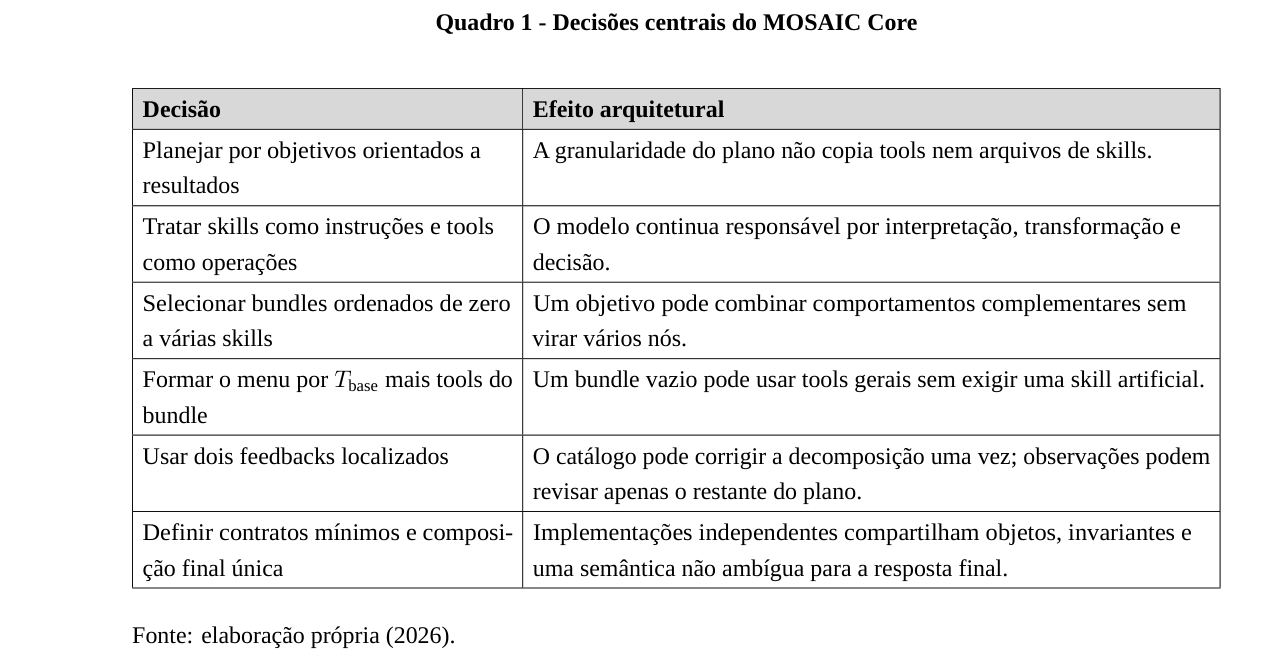
\includegraphics[width=0.97\linewidth]{figures/visual_01_p4.png}
\end{figure}

\subsection*{1.4 Escopo e modelo de confiança}

O MOSAIC Core é uma especificação técnica, não uma implementação de produção. O perfil assume:


\noindent \textbullet{} catálogo de skills confiável; \textbullet{} registro de tools confiável; \textbullet{} execução em modo YOLO, sem uma fronteira de autorização definida pelo artigo; \textbullet{} modelo capaz de seguir instruções, produzir saídas estruturadas e chamar tools; \textbullet{} estado suficiente para preservar resultados e observações entre objetivos.\par

Não fazem parte do núcleo: defesas contra prompt injection, sandbox, least privilege, confirmação de efeitos, política de credenciais, retries, idempotência, compensação de ações, execução distribuída, scripts e recursos auxiliares de Agent Skills, treinamento de retrievers, implementação de código e avaliação experimental. Esses itens são relevantes em outros recortes, mas não são necessários para especificar a composição many-to-many proposta aqui.


\subsection*{1.5 Status normativo e versão do perfil}

Este documento define o\textbf{ MOSAIC Core Profile 0.1}. Os verbos\textit{ deve} e\textit{ não deve} indicam requisitos de conformidade;\textit{ pode} indica uma opção permitida; exemplos e justificativas são infor- mativos. O perfil não prescreve linguagem, biblioteca, provedor de modelo ou protocolo de tool calling. Ele prescreve apenas os objetos e invariantes necessários para que duas implementações possam ser comparadas como instâncias do mesmo núcleo.


% Source PDF page 5

\section*{2 TRABALHOS RELACIONADOS}

\subsection*{2.1 Agent Skills}

A especificação Agent Skills define uma skill como um diretório que contém ao me- nos um arquivo\texttt{ SKILL.md}, formado por frontmatter YAML e body em Markdown.\texttt{ name} e\texttt{ description} são obrigatórios;\texttt{ allowed-tools} é opcional e experimental. A especi- ficação também prevê\texttt{ scripts/},\texttt{ references/} e\texttt{ assets/}, carregados por divulgação progressiva quando necessários (AGENT SKILLS, 2026). O MOSAIC adota o arquivo\texttt{ SKILL.md} como fonte canônica, mas define um perfil reduzido. O núcleo lê\texttt{ name},\texttt{ description},\texttt{ allowed-tools} e o body. Os diretórios opcionais continuam válidos no ecossistema Agent Skills, porém não são necessários para a arquitetura descrita neste artigo e, por isso, ficam fora do perfil central.


Essa delimitação evita afirmar compatibilidade operacional com recursos que o executor mínimo não carrega. O objetivo é compatibilidade no nível da representação de instruções, não uma implementação completa de todos os recursos do padrão.


\subsection*{2.2 SkillRouter e SkillRet}

O SkillRouter investiga roteamento em catálogos grandes e mostra que o body da skill contém sinal decisivo para distinguir itens funcionalmente próximos. Sua arquitetura usa recupe- ração de alta cobertura seguida de reranking que lê o conteúdo integral da skill (ZHENG et al., 2026). O SkillRet amplia o problema de retrieval para uma biblioteca realista de milhares de skills e reforça que selecionar instruções relevantes em catálogos grandes é uma tarefa própria, distinta do uso de tools (CHO; KANG; KIM, 2026). O MOSAIC incorpora uma exigência arquitetural desses trabalhos: o segundo estágio de seleção deve ser body-aware. A proposta não exige um retriever específico. Busca lexical, embeddings, modelos treinados ou combinações híbridas são alternativas de implementação. O requisito conceitual é que o roteamento final não dependa apenas do nome e da descrição.


\subsection*{2.3 SkillWeaver}

O SkillWeaver formaliza a composição de skills por meio de decomposição, retrieval e construção de um DAG. Sua Skill-Aware Decomposition devolve ao planejador sinais do catálogo para corrigir a decomposição inicial (GAO, 2026). Essa interação entre planejamento e retrieval é adotada pelo MOSAIC. A diferença está na unidade de composição. No SkillWeaver, a decomposição procura subtarefas atômicas associadas a skills individuais. No MOSAIC, o nó representa um resultado intermediário e pode receber um bundle de instruções. O feedback do catálogo pode revelar um resultado ausente ou uma dependência inadequada, mas não deve transformar cada skill candidata em um novo nó.


% Source PDF page 6

\subsection*{2.4 ReAct e Toolformer}

ReAct organiza a resolução de tarefas como uma alternância entre decisão, ação e ob- servação, permitindo que novas informações mudem os próximos passos (YAO et al., 2023). Toolformer explora quando chamadas de APIs acrescentam informação ou capacidade externa ao modelo (SCHICK et al., 2023). Ambos sustentam uma separação útil: o modelo interpreta e decide; a tool executa uma operação com contrato observável. O MOSAIC usa essa separação dentro de cada objetivo. O executor pode produzir o resultado diretamente ou alternar chamadas de tools e observações até que os critérios de conclusão sejam atendidos. Uma chamada de tool não se torna automaticamente um nó do plano.


\subsection*{2.5 Evidência recente sobre skills, bundles e menus de tools}

SkillsBench trata skills como pacotes de conhecimento procedural e mostra que instruções focadas podem ser mais úteis do que documentação acumulada (LI et al., 2026). SkillMOO trata bundles como objetos passíveis de poda e substituição, reforçando que adicionar instruções indis- criminadamente não é equivalente a melhorar o agente (GONG et al., 2026). ToolMenuBench, por sua vez, transforma a construção do menu visível de tools em um problema de primeira classe (BABU; IYER, 2026).


Esses trabalhos ajudam a posicionar o MOSAIC, mas não são incorporados como novos


\begin{figure}[H]
\centering
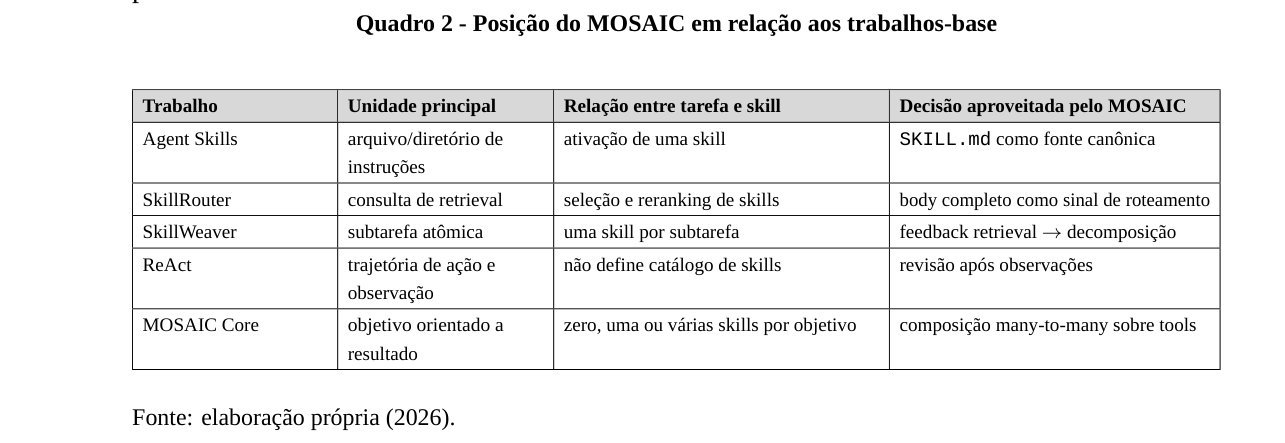
\includegraphics[width=0.97\linewidth]{figures/visual_02_p6.png}
\end{figure}

\section*{3 MODELO CONCEITUAL}

\subsection*{3.1 Vocabulário mínimo}

A arquitetura usa os conceitos do Quadro 3.


% Source PDF page 7

\begin{figure}[H]
\centering
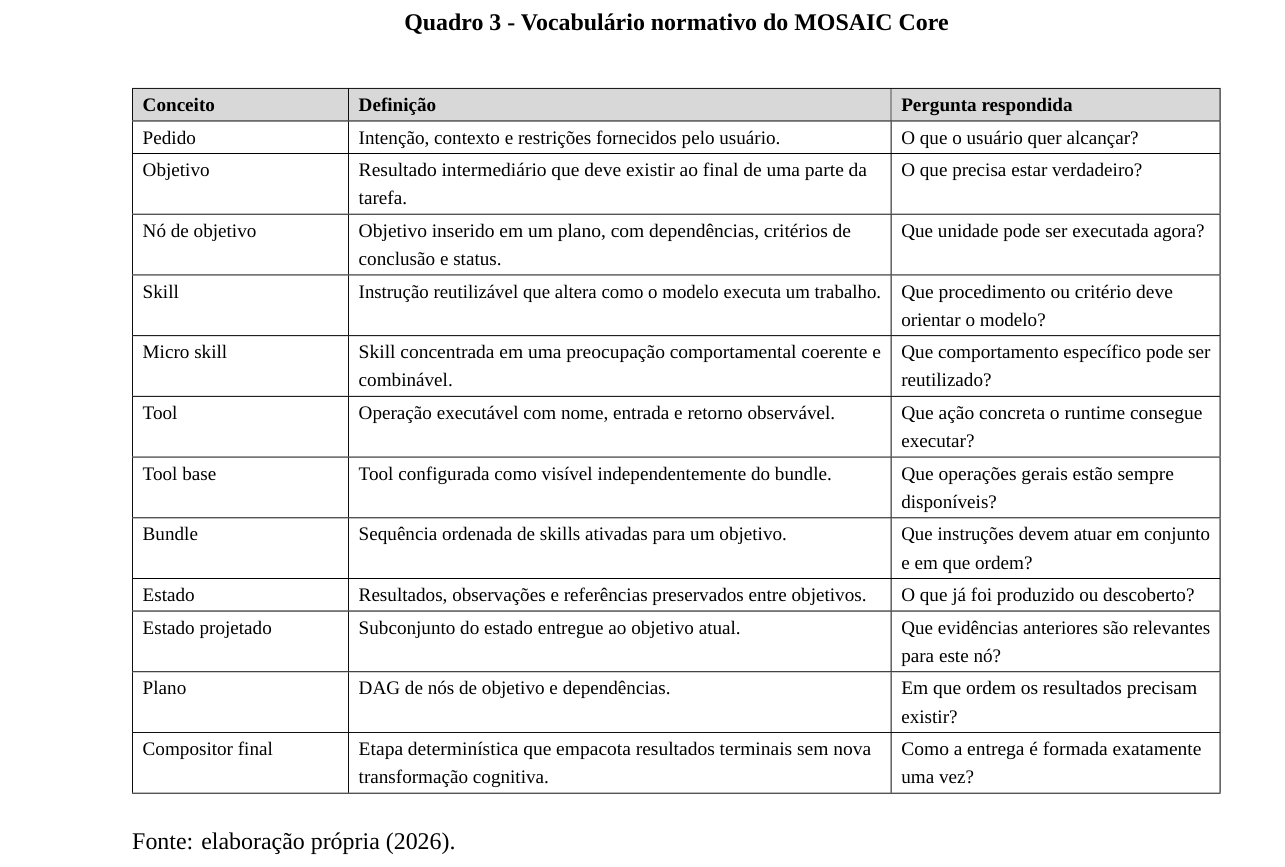
\includegraphics[width=0.97\linewidth]{figures/visual_03_p7.png}
\end{figure}

\begin{figure}[H]
\centering
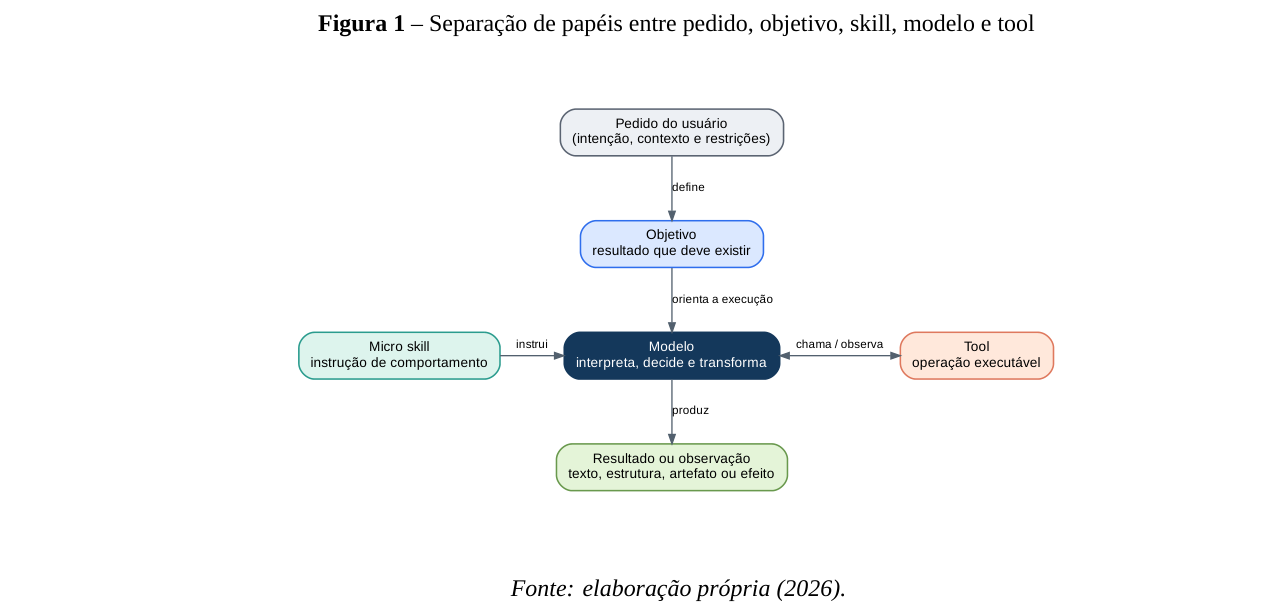
\includegraphics[width=0.97\linewidth]{figures/visual_04_p7.png}
\end{figure}

A separação da Figura 1 é normativa para a arquitetura. O objetivo descreve o resultado; a skill orienta o comportamento; a tool executa uma operação; o modelo decide como combinar esses elementos. Nenhum dos conceitos substitui os demais.


% Source PDF page 8

\subsection*{3.2 O que torna uma skill “micro”}

“Micro” não significa uma única linha, uma única chamada ou uma única tool. Uma micro skill é pequena em responsabilidade, não necessariamente em número de passos. Ela deve atender a quatro propriedades:


\noindent 1.\textbf{ Coerência:} ensina uma preocupação comportamental identificável, como fundamentar afirmações em evidências ou comparar alternativas sob critérios explícitos. 2.\textbf{ Reutilização:} pode ser aplicada a mais de um pedido ou objetivo sem depender de um workflow inteiro. 3.\textbf{ Composição:} pode atuar ao lado de outras skills sem assumir controle exclusivo da tarefa. 4.\textbf{ Carga integral:} seu body é conciso o suficiente para ser carregado completo quando selecionado.\par

\texttt{evidence-grounded-summary} é micro porque ensina como ligar afirmações a dados.\texttt{ uncertainty-reporting} é micro porque ensina como explicitar premissas e li- mitações.\texttt{ latest-document-reading} também pode ser micro mesmo usando\texttt{ list} e \texttt{read}, pois sua responsabilidade coerente é identificar e disponibilizar o documento correto.


Em contraste,\texttt{ financial-agent-that-does-everything} mistura descoberta, leitura, análise, decisão, redação e persistência.\texttt{ use-read-when-reading} apenas repete o nome da tool e não acrescenta comportamento. O primeiro é amplo demais; o segundo é vazio demais.


\subsection*{3.3 Granularidade do objetivo}

Um objetivo descreve um resultado, não uma sequência de operações. A frase “obter o relatório financeiro mais recente e válido” é um objetivo. A frase “chamar\texttt{ list}, ordenar datas e chamar\texttt{ read}” é uma trajetória de execução. Uma nova etapa é justificada quando pelo menos uma das condições abaixo ocorre:


\noindent \textbullet{} o resultado será consumido por outro objetivo; \textbullet{} uma observação externa pode mudar o restante do plano; \textbullet{} uma parte possui critério de conclusão próprio; \textbullet{} duas partes podem ser executadas independentemente; \textbullet{} o usuário pediu resultados ou artefatos separados.\par

A existência de uma tool ou de uma skill não é, sozinha, motivo para criar um nó. Listar arquivos, comparar nomes e ler um documento podem ocorrer dentro do mesmo objetivo. Da mesma forma, aplicar duas skills cognitivas ao mesmo conjunto de dados não exige dois objetivos.


% Source PDF page 9

\subsection*{3.4 Relações many-to-many}

Considere um plano P = (G, E), em que G é o conjunto de objetivos e E contém dependências acíclicas. Para cada objetivo g, o seletor produz um bundle ordenado:


B(g) = ⟨s1, . . . , sk⟩, 0 ≤k ≤Kmax. (1) Kmax é um limite pequeno configurado pelo runtime. Ele não define quantas skills existem no catálogo; apenas impede que um único objetivo acumule instruções demais. Cada skill s pode declarar um conjunto A(s) de tools em\texttt{ allowed-tools}. O menu visível para o objetivo é:


T(g) = Tbase ∪ [ s∈B(g) A(s). (2) Tbase é o conjunto de tools gerais que o runtime decide expor a todos os objetivos. No perfil YOLO máximo, pode-se definir Tbase = Tregistry, tornando todas as tools registradas sempre visíveis. Em um perfil reduzido,\texttt{ calculator} pode ser base enquanto integrações específicas, como\texttt{ slack\_send\_message}, entram pelo bundle. A fórmula resolve um caso importante: se B(g) = ∅, o objetivo ainda pode usar Tbase. Portanto, uma operação geral não exige uma skill artificial. Se nenhuma tool for necessária, o modelo conclui o objetivo cognitivamente.


\begin{figure}[H]
\centering
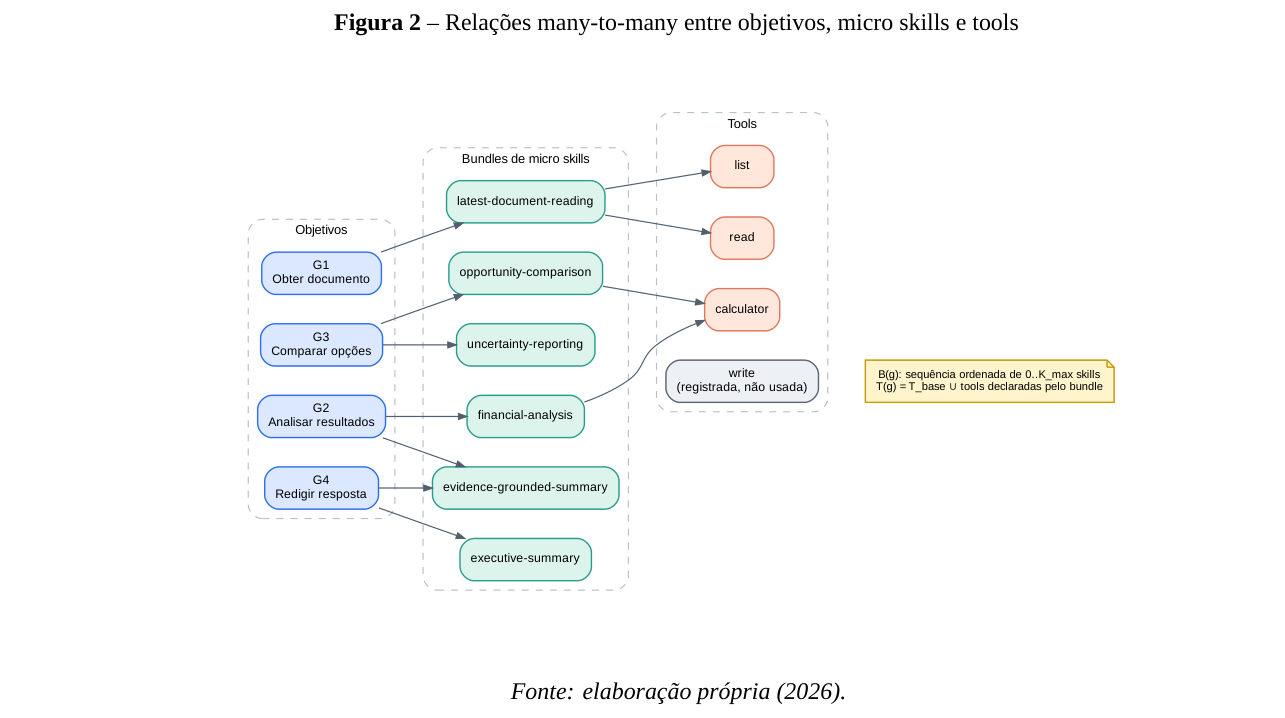
\includegraphics[width=0.97\linewidth]{figures/visual_05_p9.png}
\end{figure}

% Source PDF page 10

A Figura 2 também mostra que uma skill pode orientar vários objetivos, que um objetivo pode combinar várias skills e que a mesma tool pode aparecer sob procedimentos diferentes. A semântica da operação permanece estável; o comportamento muda conforme o bundle.


\subsection*{3.5 Semântica do bundle ordenado}

O bundle é uma sequência, não um conjunto sem ordem. O executor injeta bodies no contexto em uma ordem observável, e essa ordem pode afetar o modelo. Para evitar que duas implementações igualmente conformes usem convenções incompatíveis, o MOSAIC Core 0.1 define a regra mínima abaixo:


\noindent \textbullet{} o reranker produz uma ordem de aplicabilidade; \textbullet{} o seletor percorre essa ordem e retém até Kmax skills que acrescentem comportamentos distintos e necessários; \textbullet{} a ordem final do bundle preserva a posição do reranking entre as skills selecionadas; \textbullet{} empates de score são resolvidos pelo nome canônico da skill em ordem lexicográfica crescente; \textbullet{} skills redundantes, conflitantes ou fora do objetivo são omitidas; \textbullet{} o seletor pode retornar uma sequência vazia.\par

No perfil Core, a ordem de aplicabilidade é deliberadamente usada como ordem de composição. Essa é uma convenção de referência, não uma afirmação de que ela seja ótima. Uma extensão pode adotar precedência mais rica, desde que declare outra versão de perfil. Os bodies devem ser delimitados pelo nome canônico da skill para impedir fusão acidental entre instruções adjacentes.


\section*{4 ARQUITETURA MÍNIMA}

\subsection*{4.1 Visão geral}

O MOSAIC Core possui seis estágios de runtime, alimentados por um catálogo canônico e conectados por um estado compartilhado:


\noindent 1. planejador de objetivos; 2. feedback do catálogo e revisão única do plano inicial; 3. roteador de skills e seletor de bundle; 4. montagem do menu de tools; 5. executor do nó; 6. compositor final determinístico.\par

O estado preserva resultados e observações. Quando uma observação invalida uma suposição, o planejador revisa somente a parte não concluída do plano. O compositor final


% Source PDF page 11

não realiza uma segunda síntese: ele apenas entrega os resultados que já foram produzidos por objetivos terminais.


\begin{figure}[H]
\centering
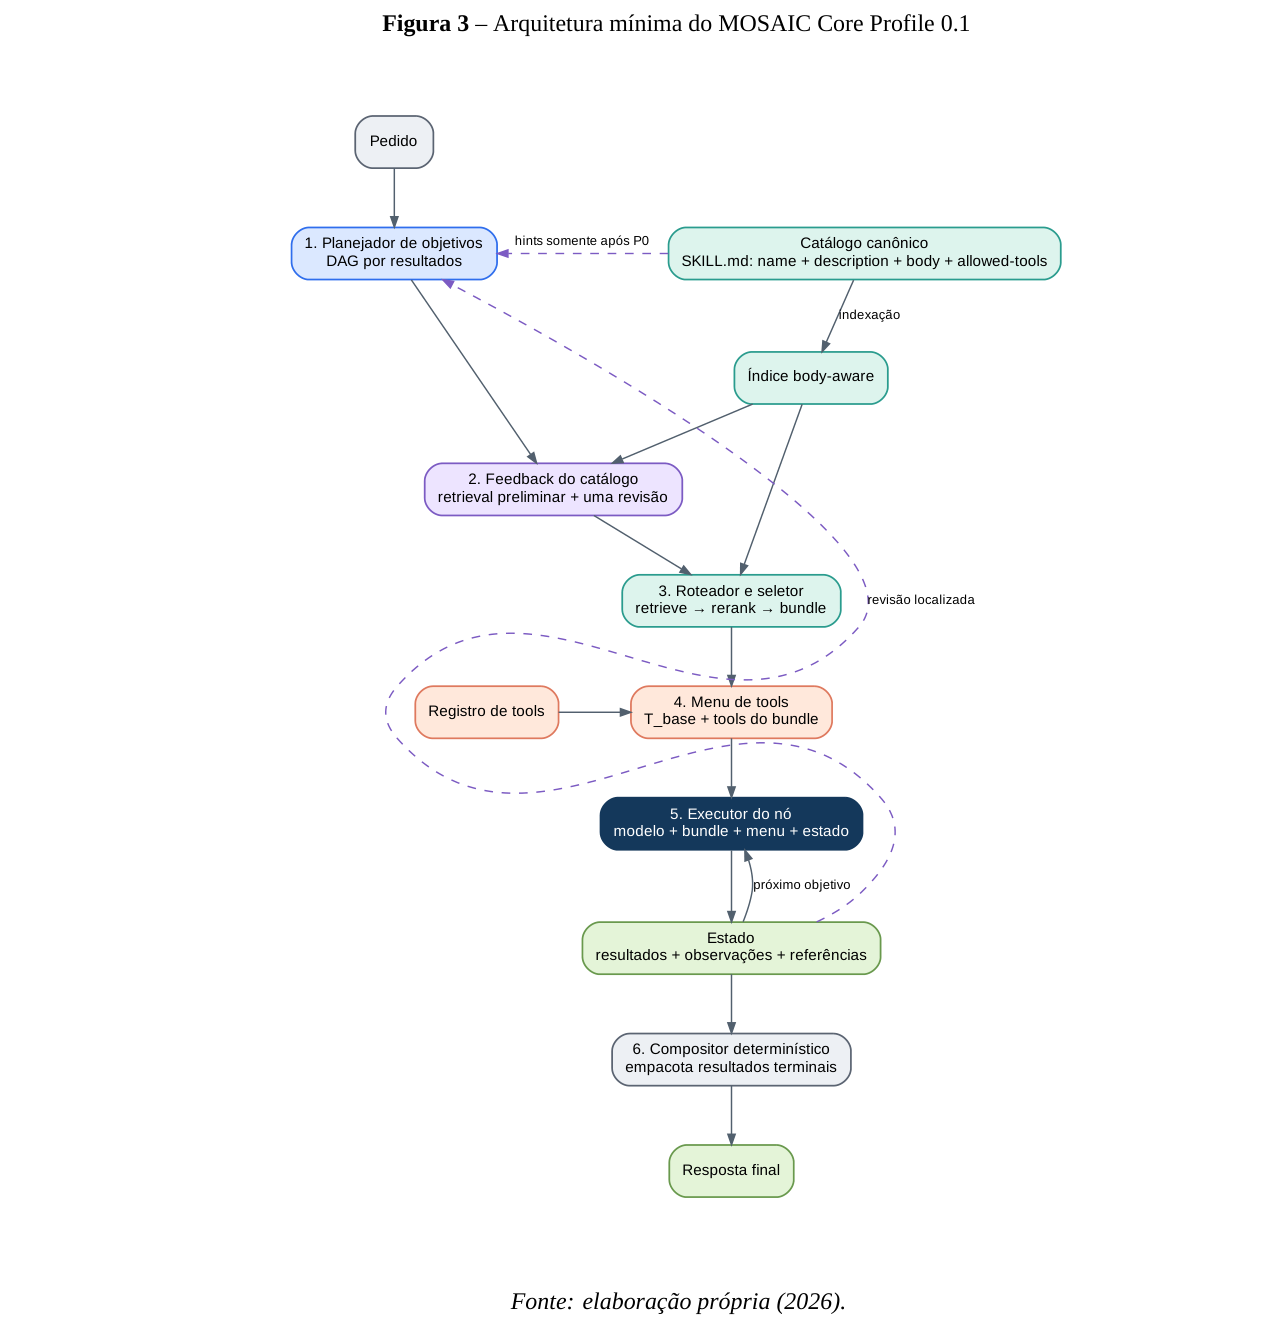
\includegraphics[width=0.97\linewidth]{figures/visual_06_p11.png}
\end{figure}

A Figura 3 separa duas responsabilidades. O catálogo prepara representações para busca; o runtime transforma um pedido em resultados. O catálogo não define a granularidade do plano, e o planner não escolhe tools diretamente.


% Source PDF page 12

\subsection*{4.2 Catálogo canônico e índice body-aware}

Cada skill é representada por um\texttt{ SKILL.md}. O núcleo mantém somente os dados necessários para recuperação e execução:


\noindent \textbullet{}\texttt{ name}; \textbullet{}\texttt{ description}; \textbullet{} body completo; \textbullet{} lista normalizada de\texttt{ allowed-tools}; \textbullet{} texto de indexação derivado deterministicamente desses campos.\par

O carregamento do catálogo é\textit{ fail-fast} para os campos do perfil Core. A implementação deve rejeitar o catálogo quando houver nome de skill duplicado, campo obrigatório ausente, body vazio ou nome de tool declarado que não exista em Tregistry. Tools repetidas em uma mesma skill são deduplicadas. Campos desconhecidos podem ser preservados, mas não alteram o núcleo. Uma versão anterior da arquitetura previa um compilador baseado em modelo para inferir \texttt{useWhen}, behaviors, outputs e outros campos. Esse componente foi removido do núcleo. A recuperação body-aware já pode operar sobre\texttt{ name},\texttt{ description} e body; o reranker lê a fonte original. Metadados inferidos podem ser úteis em implementações específicas, mas não são necessários para expressar a composição. O índice pode ser lexical, vetorial ou híbrido. O MOSAIC não fixa o mecanismo. A única exigência é preservar um caminho do resultado de retrieval até o body canônico, pois o reranking e a execução dependem das instruções reais, não apenas de resumos derivados.


\subsection*{4.3 Planejamento inicial por resultados}

O planejador recebe o pedido e produz um DAG inicial P0. Nessa primeira passagem, ele não recebe nomes de skills. Isso reduz a tendência de copiar a estrutura física do catálogo. Cada nó deve possuir:


\noindent \textbullet{} identificador único no plano; \textbullet{} objetivo orientado a resultado; \textbullet{} dependências que referenciam apenas IDs existentes; \textbullet{} critérios\texttt{ doneWhen}; \textbullet{} status inicial\texttt{ pending}.\par

Para o pedido financeiro, um plano inicial plausível é:


\noindent 1. obter o relatório mais recente e válido; 2. interpretar os resultados relevantes; 3. comparar oportunidades; 4. redigir a resposta.\par

O planner não precisa antecipar chamadas como\texttt{ list},\texttt{ read} ou\texttt{ calculator}. Essas decisões pertencem ao executor de cada nó.


% Source PDF page 13

\subsection*{4.4 Feedback do catálogo e revisão única}

Depois de P0, o runtime executa uma recuperação preliminar por objetivo. Para cada consulta, no máximo Khint candidatas são convertidas em hints curtas, fundamentadas no body. As hints podem revelar:


\noindent \textbullet{} vocabulário do domínio que não apareceu no pedido; \textbullet{} um resultado intermediário ausente; \textbullet{} uma divisão artificial; \textbullet{} uma dependência inadequada.\par

O planner recebe essas hints e pode produzir P1. A revisão ocorre uma vez antes da execução. Depois dela, o roteamento é refeito para os objetivos finais. Esse fluxo evita revisar um plano antes de gerar os sinais do catálogo.


\begin{figure}[H]
\centering
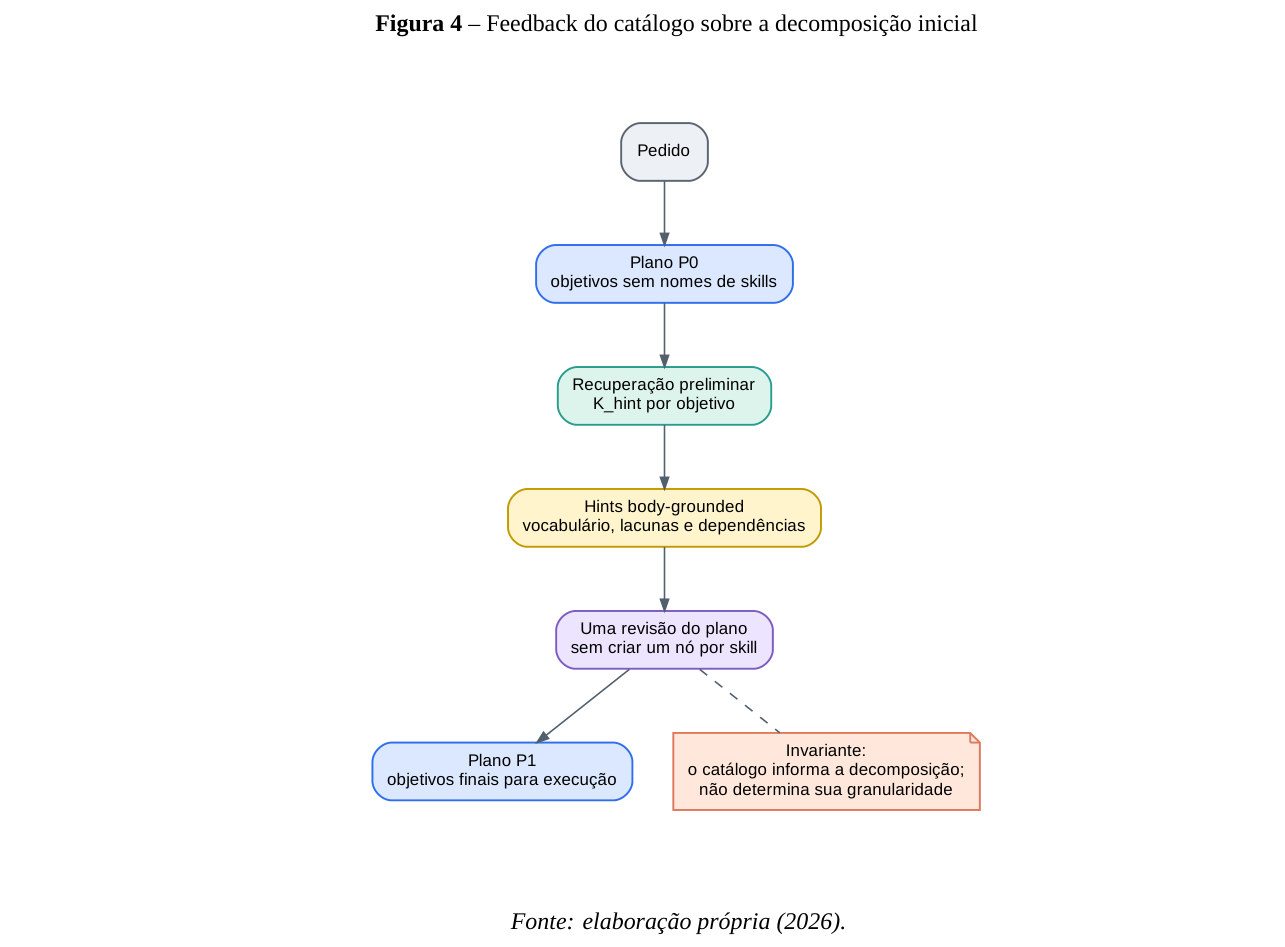
\includegraphics[width=0.97\linewidth]{figures/visual_07_p13.png}
\end{figure}

A regra de controle é simples: uma skill pode revelar que “analisar” e “resumir” são resultados semanticamente diferentes, mas sua mera existência não cria um nó. O catálogo informa o planner; não governa sua granularidade.


% Source PDF page 14

\subsection*{4.5 Retrieval, reranking e seleção do bundle}

Para cada objetivo pronto, o roteador constrói uma consulta com:


\noindent \textbullet{} descrição do objetivo; \textbullet{} critérios\texttt{ doneWhen}; \textbullet{} termos relevantes do pedido original; \textbullet{} saídas necessárias dos objetivos anteriores.\par

O primeiro estágio privilegia cobertura e retorna até Kretrieve candidatas. O segundo compara as candidatas usando o body completo. Em seguida, o seletor percorre a lista reranqueada e retém, até Kmax, apenas as skills que acrescentam comportamentos distintos e necessários.


\begin{figure}[H]
\centering
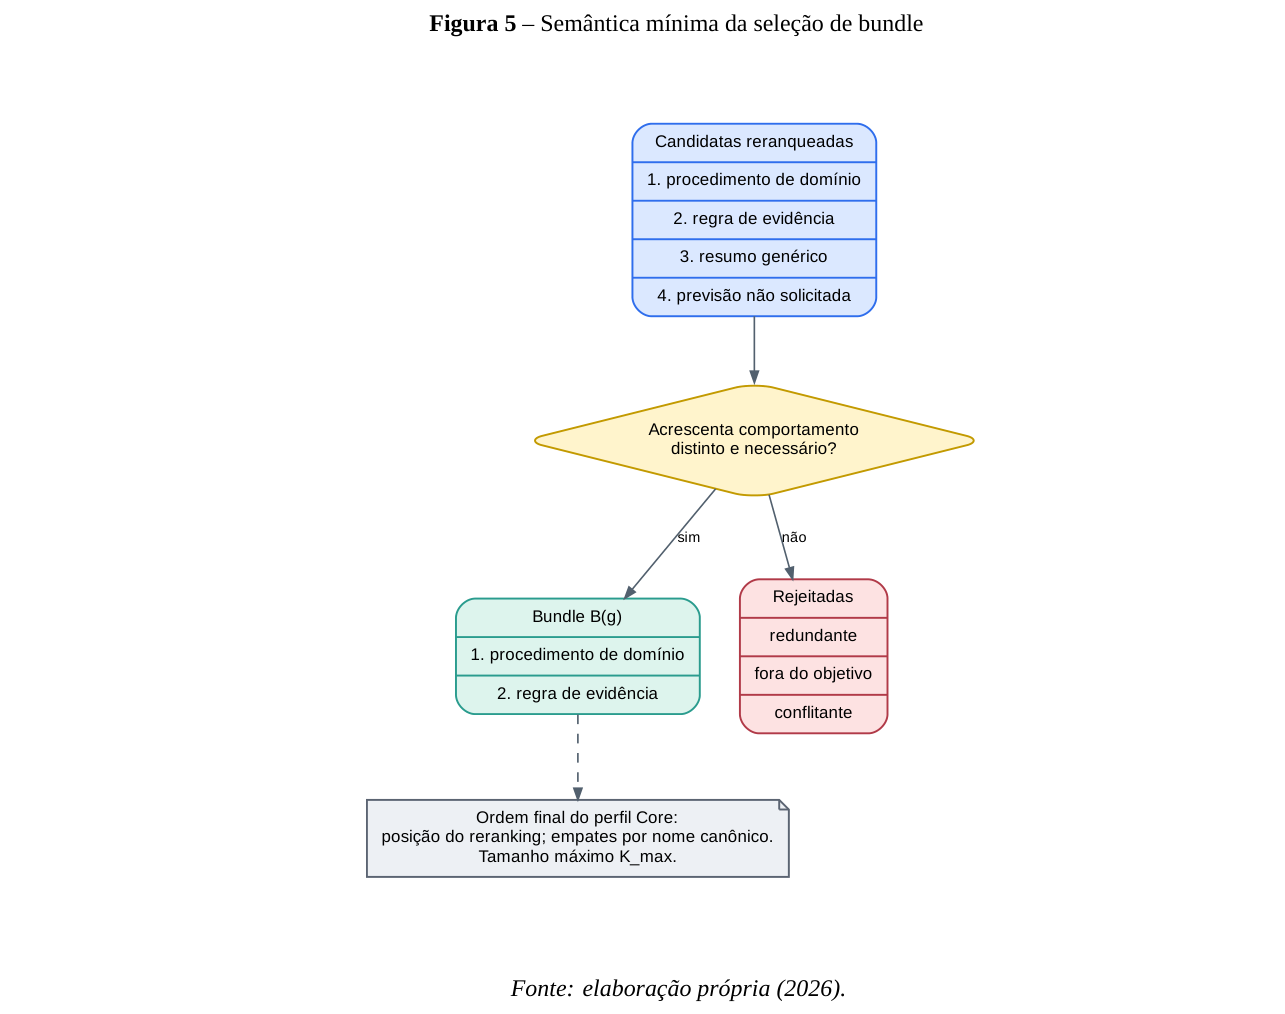
\includegraphics[width=0.97\linewidth]{figures/visual_08_p14.png}
\end{figure}

A seleção é baseada no comportamento ensinado pela skill. Uma skill não deve ser escolhida apenas porque declara uma tool útil. Se uma operação geral já estiver em Tbase, ela continua disponível mesmo quando nenhuma skill é selecionada.


% Source PDF page 15

\subsection*{4.6 Montagem do menu de tools}

Após a seleção, o runtime calcula T(g) pela fórmula apresentada anteriormente. Não existe um tool router independente no núcleo. Essa remoção é deliberada: um segundo roteador duplicaria a decisão de relevância antes que a hipótese básica fosse demonstrada.


\begin{figure}[H]
\centering
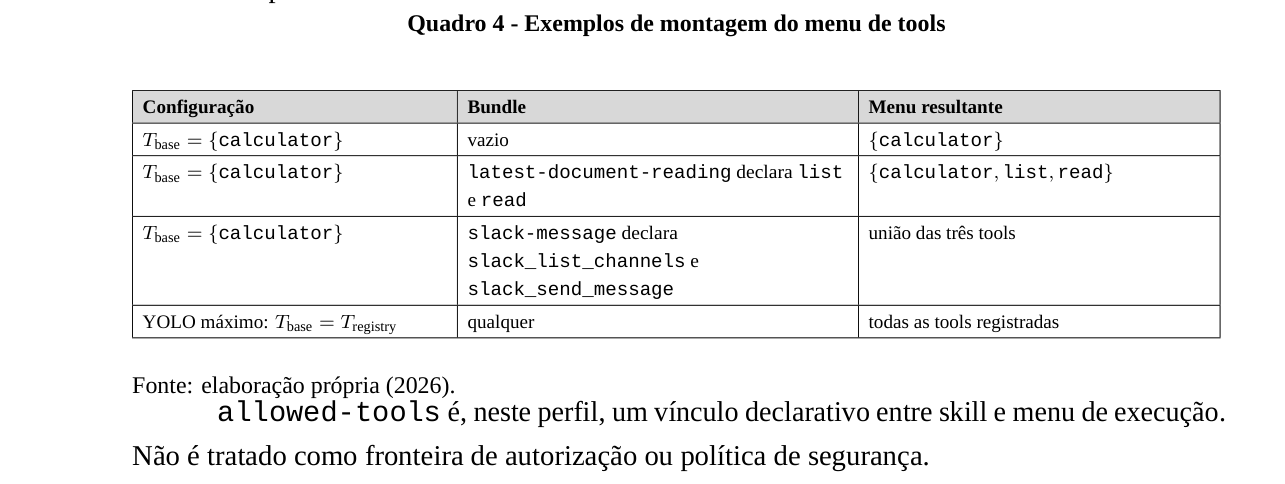
\includegraphics[width=0.97\linewidth]{figures/visual_09_p15.png}
\end{figure}

\subsection*{4.7 Montagem do contexto e projeção de estado}

O executor recebe somente o contexto necessário para o objetivo atual. A montagem deve seguir a ordem estável abaixo:


\noindent 1. instruções do runtime; 2. pedido original e restrições globais; 3. objetivo atual e seus critérios\texttt{ doneWhen}; 4. estado projetado; 5. bodies das skills do bundle, cada um entre delimitadores que contenham o nome canônico; 6. schemas das tools de T(g).\par

Por padrão, o estado projetado de um objetivo contém:


\noindent \textbullet{} saídas dos ancestrais transitivos do nó no DAG; \textbullet{} observações explicitamente referenciadas pelo objetivo ou por uma revisão; \textbullet{} restrições globais do pedido; \textbullet{} referências para artefatos necessários à execução.\par

Resultados de ramos sem dependência causal com o objetivo atual são omitidos, salvo quando o plano os referencia explicitamente. Essa regra reduz contexto e torna a projeção auditável sem introduzir um novo subsistema de memória.


% Source PDF page 16

\subsection*{4.8 Executor do nó}

O modelo pode concluir diretamente ou chamar tools. Uma observação volta ao mesmo nó; ela não cria automaticamente um novo objetivo. O nó termina quando o resultado satisfaz seus critérios de conclusão, quando uma observação solicita revisão estrutural ou quando o runtime encerra a trajetória por limite ou impossibilidade explícita. Lnode define o número máximo de turnos de modelo/tool dentro de um nó. O limite é um parâmetro de controle, não uma taxonomia de erros. Se\texttt{ doneWhen} não foi satisfeito e o modelo não propõe uma ação útil, o nó termina como\texttt{ blocked}. Saídas estruturalmente inválidas ou falhas terminais podem produzir\texttt{ failed}.


\begin{figure}[H]
\centering
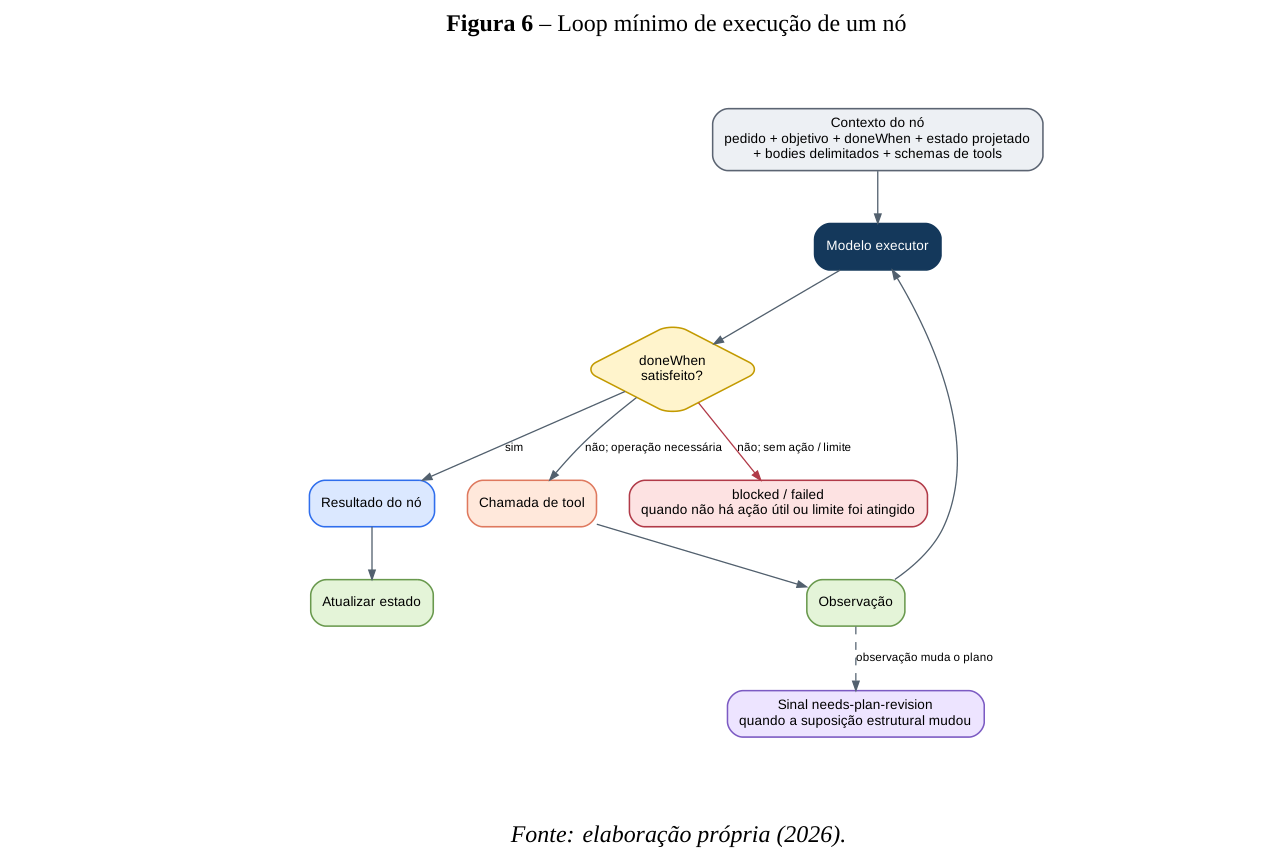
\includegraphics[width=0.97\linewidth]{figures/visual_10_p16.png}
\end{figure}

\subsection*{4.9 Ciclo de vida do nó e revisão localizada}

O status de um nó pertence ao conjunto:


\{\texttt{pending},\texttt{ ready},\texttt{ running},\texttt{ completed},\texttt{ needs\_revision},\texttt{ blocked},\texttt{ failed}\}. (3) Um nó\texttt{ pending} torna-se\texttt{ ready} quando todas as dependências estão\texttt{ completed}. O scheduler o coloca em\texttt{ running}. A satisfação de\texttt{ doneWhen} leva a\texttt{ completed}. Uma


% Source PDF page 17

observação que invalide uma suposição estrutural produz\texttt{ needs\_revision}; a ausência de ação útil ou o esgotamento de Lnode produz\texttt{ blocked}; uma falha terminal produz\texttt{ failed}.


\begin{figure}[H]
\centering
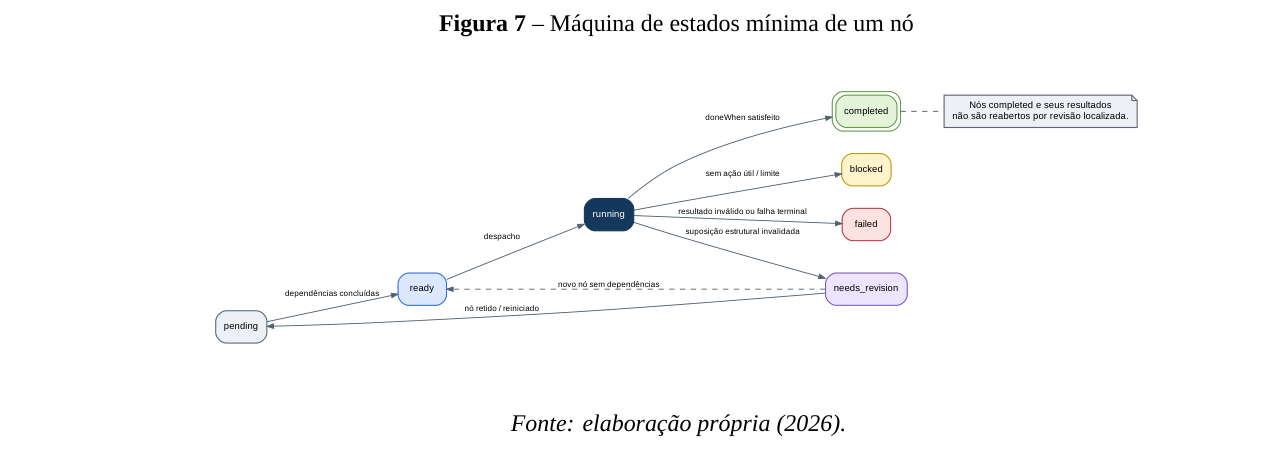
\includegraphics[width=0.97\linewidth]{figures/visual_11_p17.png}
\end{figure}

Quando ocorre revisão:


\noindent \textbullet{} objetivos\texttt{ completed} permanecem concluídos e seus resultados permanecem no estado; \textbullet{} somente o nó atual ainda incompleto e objetivos não iniciados podem ser retidos, substitu- ídos, removidos ou inseridos; \textbullet{} IDs de nós sobreviventes permanecem estáveis; \textbullet{} dependentes de um nó removido devem ser removidos ou reconectados explicitamente; \textbullet{} o plano revisado deve continuar acíclico e referenciar apenas IDs existentes; \textbullet{} o nó atual pode ser mantido com o mesmo ID e reiniciado como\texttt{ pending}, ou substituído quando a nova decomposição exigir outra unidade de resultado.\par

Rmax limita o número de revisões localizadas em uma execução. O artigo não prescreve um valor universal; o runtime deve declarar o valor usado. Essa guarda impede ciclos infinitos sem transformar o núcleo em um protocolo completo de recuperação.


\subsection*{4.10 Composição da resposta final}

Objetivos terminais produzem o conteúdo semanticamente final. Quando a tarefa exige síntese, redação ou decisão, o plano deve conter um objetivo terminal responsável por essa transformação, como G4 no exemplo financeiro. A função\texttt{ compor\_resposta} não chama o modelo e não aplica skills novamente. Ela seleciona resultados de nós terminais marcados para entrega, ordena-os de forma estável pela ordem topológica e empacota texto, referências de artefatos e efeitos observáveis. Assim, a resposta é produzida exatamente uma vez e o trace identifica qual objetivo realizou a síntese.


% Source PDF page 18

\begin{figure}[H]
\centering
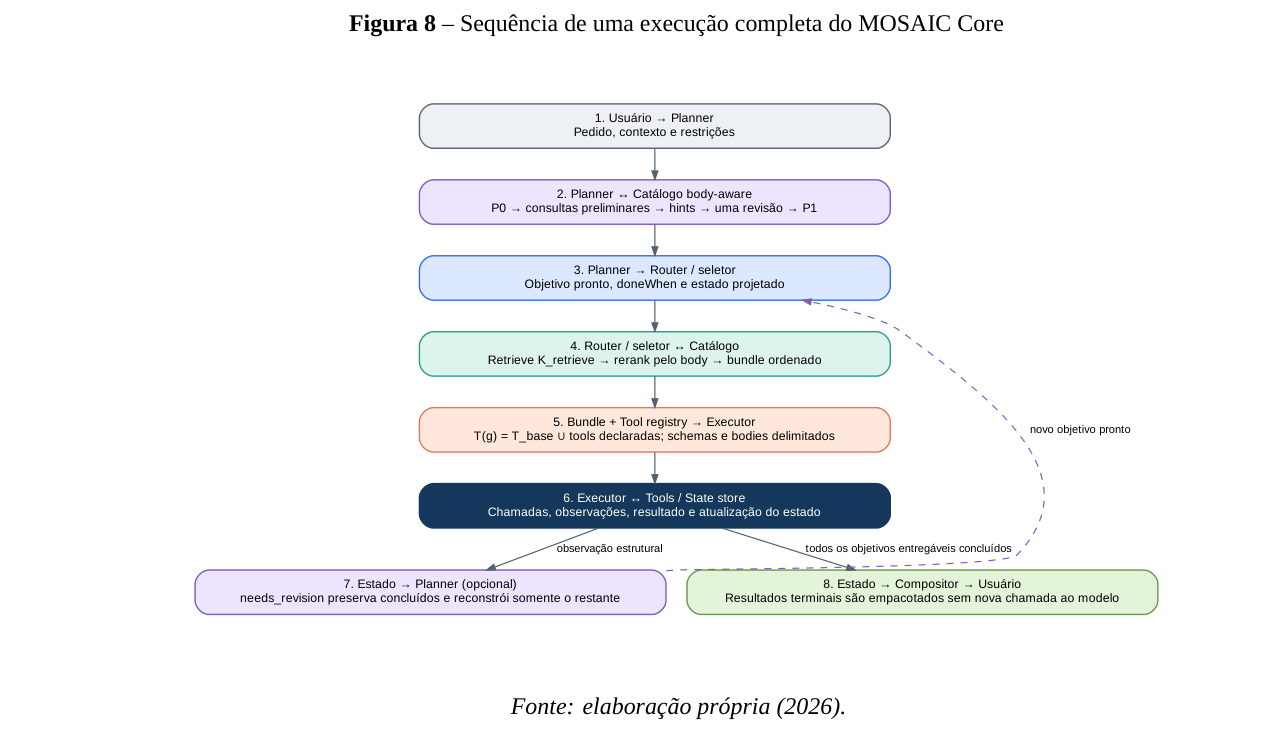
\includegraphics[width=0.97\linewidth]{figures/visual_12_p18.png}
\end{figure}

\section*{5 ALGORITMO CENTRAL}

A arquitetura pode ser expressa pelo algoritmo abstrato abaixo. Ele especifica a ordem das decisões sem fixar linguagem, biblioteca, modelo ou protocolo de erros.


\textbf{Algoritmo 1 - Execução do MOSAIC Core Profile 0.1}


\begin{Verbatim}[breaklines=true,breakanywhere=true,fontsize=\small]
entrada:
\end{Verbatim}

\begin{Verbatim}[breaklines=true,breakanywhere=true,fontsize=\small]
pedido q
catálogo de skills S
registro de tools T_registry
conjunto base T_base
K_retrieve, K_hint, K_max
limite por nó L_node
limite de revisões R_max
\end{Verbatim}

\begin{Verbatim}[breaklines=true,breakanywhere=true,fontsize=\small]
validar_catalogo_e_registro(S, T_registry, T_base)
P0 <- planejar_objetivos(q)
// sem nomes de skills
validar_dag(P0)
H
<- recuperar_hints_body_aware(P0, S, K_hint)
P
<- revisar_uma_vez(q, P0, H)
validar_dag(P)
\end{Verbatim}

\begin{Verbatim}[breaklines=true,breakanywhere=true,fontsize=\small]
estado <- vazio
revisoes <- 0
\end{Verbatim}

% Source PDF page 19

\begin{Verbatim}[breaklines=true,breakanywhere=true,fontsize=\small]
enquanto houver objetivo não terminal em P:
\end{Verbatim}

\begin{Verbatim}[breaklines=true,breakanywhere=true,fontsize=\small]
g <- próximo objetivo pending cujas dependências estão completed
marcar(g, ready)
C <- recuperar_e_reranquear(g, q, projetar_estado(g, P, estado),
\end{Verbatim}

\begin{Verbatim}[breaklines=true,breakanywhere=true,fontsize=\small]
S, K_retrieve)
B <- selecionar_bundle_ordenado(C, K_max)
T <- T_base união tools_declaradas(B)
contexto <- montar_contexto(q, g, projetar_estado(g, P, estado), B, T)
outcome <- executar_ate_terminal(contexto, L_node)
\end{Verbatim}

\begin{Verbatim}[breaklines=true,breakanywhere=true,fontsize=\small]
se outcome.status = completed:
\end{Verbatim}

\begin{Verbatim}[breaklines=true,breakanywhere=true,fontsize=\small]
estado <- incorporar(outcome.resultado, outcome.observacoes)
marcar(g, completed)
\end{Verbatim}

\begin{Verbatim}[breaklines=true,breakanywhere=true,fontsize=\small]
senão se outcome.status = needs_revision e revisoes < R_max:
\end{Verbatim}

\begin{Verbatim}[breaklines=true,breakanywhere=true,fontsize=\small]
estado <- incorporar(outcome.observacoes)
P <- revisar_objetivo_atual_e_restantes(P, g, estado)
validar_dag(P)
revisoes <- revisoes + 1
\end{Verbatim}

\begin{Verbatim}[breaklines=true,breakanywhere=true,fontsize=\small]
senão:
\end{Verbatim}

\begin{Verbatim}[breaklines=true,breakanywhere=true,fontsize=\small]
registrar outcome como blocked ou failed
\end{Verbatim}

\begin{Verbatim}[breaklines=true,breakanywhere=true,fontsize=\small]
retornar compor_resposta_deterministicamente(q, P, estado)
\end{Verbatim}

O algoritmo mantém seis invariantes de conformidade:


\noindent 1. objetivos descrevem resultados, não chamadas de tools nem nomes de skills; 2. o planner inicial não depende dos nomes das skills; 3. o bundle pode conter zero, uma ou várias skills e possui ordem observável; 4. tools gerais podem existir fora das skills por meio de Tbase; 5. o body canônico é usado tanto no reranking quanto na execução; 6. uma revisão preserva nós concluídos e altera apenas o nó atual incompleto e a parte ainda não iniciada do plano.\par

Uma implementação que preserve esses invariantes e os contratos do Apêndice A pode variar livremente em modelo, índice, linguagem, formato de serialização e protocolo de tool calling.


\section*{6 PERFIL MOSAIC CORE PARA SKILL.MD}

\subsection*{6.1 Subconjunto suportado}

O perfil mínimo usa o subconjunto do Quadro 5.


% Source PDF page 20

\begin{figure}[H]
\centering
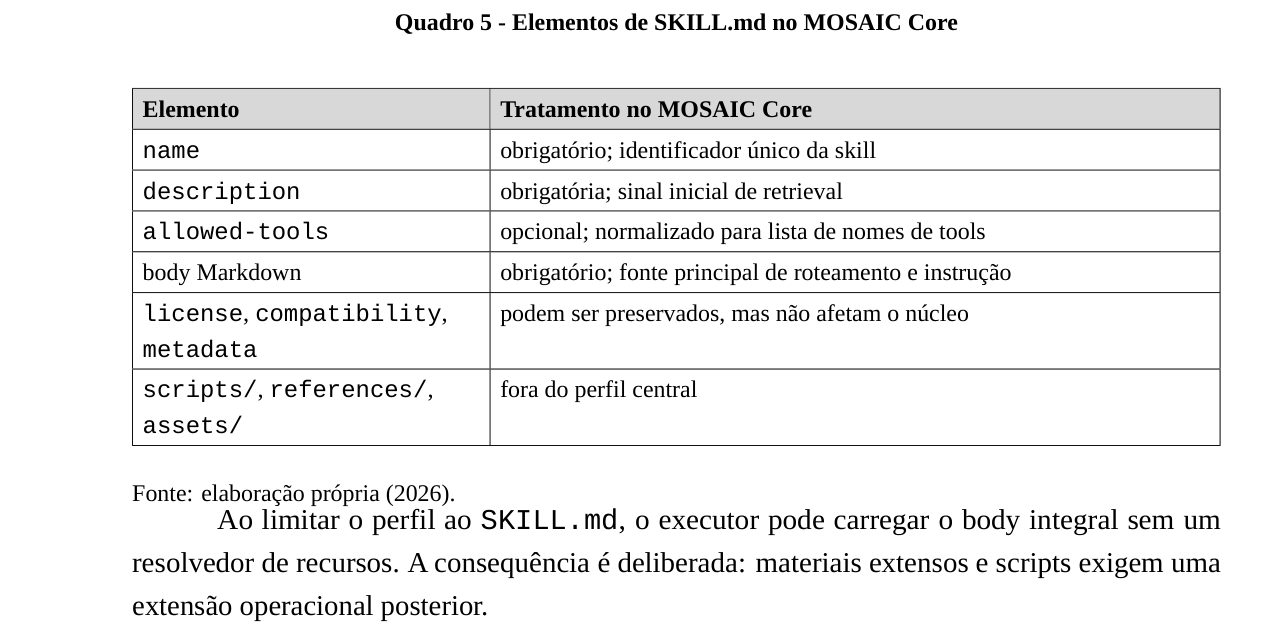
\includegraphics[width=0.97\linewidth]{figures/visual_13_p20.png}
\end{figure}

\subsection*{6.2 Gramática e normalização de allowed-tools}

A forma canônica do MOSAIC Core é uma sequência YAML:


\begin{Verbatim}[breaklines=true,breakanywhere=true,fontsize=\small]
allowed-tools:
\end{Verbatim}

\begin{Verbatim}[breaklines=true,breakanywhere=true,fontsize=\small]
- calculator
- read
\end{Verbatim}

Para compatibilidade de ingestão, uma implementação pode aceitar um escalar com nomes separados por espaços, como\texttt{ allowed-tools: list read}. O parser deve normalizar as duas formas para\texttt{ string[]}, remover duplicatas e preservar a ordem de primeira ocorrência. Nomes de tools são identificadores exatos, sensíveis a caixa quando o registro também o for. Uma referência que não resolva em Tregistry invalida o carregamento do catálogo.


\subsection*{6.3 Estrutura recomendada do body}

O formato do body permanece livre, mas uma micro skill legível tende a responder cinco perguntas:


\noindent 1. qual comportamento ela ensina; 2. quando deve ser usada; 3. quando não deve ser usada; 4. qual procedimento ou critério deve ser seguido; 5. como reconhecer a conclusão.\par

Uma estrutura recomendada é:


\begin{Verbatim}[breaklines=true,breakanywhere=true,fontsize=\small]
# Nome legível
\end{Verbatim}

% Source PDF page 21

\begin{Verbatim}[breaklines=true,breakanywhere=true,fontsize=\small]
## Purpose
Explique a preocupação comportamental da skill.
\end{Verbatim}

\begin{Verbatim}[breaklines=true,breakanywhere=true,fontsize=\small]
## Use this skill when
- descreva situações aplicáveis.
\end{Verbatim}

\begin{Verbatim}[breaklines=true,breakanywhere=true,fontsize=\small]
## Do not use this skill when
- descreva situações não aplicáveis.
\end{Verbatim}

\begin{Verbatim}[breaklines=true,breakanywhere=true,fontsize=\small]
## Procedure
1. descreva o método ou os critérios.
\end{Verbatim}

\begin{Verbatim}[breaklines=true,breakanywhere=true,fontsize=\small]
## Completion
Descreva o resultado esperado.
\end{Verbatim}

Os títulos não são obrigatórios. O requisito é semântico: o body precisa acrescentar comportamento que o nome da tool ou uma descrição genérica não expressam.


\subsection*{6.4 Exemplo cognitivo com tool opcional}

\begin{Verbatim}[breaklines=true,breakanywhere=true,fontsize=\small]
---
name: financial-analysis
description: Interprets reported financial results, compares periods,
\end{Verbatim}

\begin{Verbatim}[breaklines=true,breakanywhere=true,fontsize=\small]
and identifies material business changes. Use when financial evidence
must be understood rather than merely copied.
allowed-tools:
\end{Verbatim}

\begin{Verbatim}[breaklines=true,breakanywhere=true,fontsize=\small]
- calculator
---
\end{Verbatim}

\begin{Verbatim}[breaklines=true,breakanywhere=true,fontsize=\small]
# Financial Analysis
Compare period, units, revenue, margins, cash generation and material
\end{Verbatim}

\begin{Verbatim}[breaklines=true,breakanywhere=true,fontsize=\small]
costs.
Separate recurring changes from one-time events.
Connect claims to reported figures and state missing information.
Use calculator only when a derived metric is necessary.
Completion: the main changes, their evidence and the principal
\end{Verbatim}

\begin{Verbatim}[breaklines=true,breakanywhere=true,fontsize=\small]
limitation
are explicit.
\end{Verbatim}

A skill continua cognitiva: seu principal valor é o método de análise.\texttt{ calculator} apenas acrescenta uma operação possível.


\subsection*{6.5 Exemplo de uma skill com várias tools}

\begin{Verbatim}[breaklines=true,breakanywhere=true,fontsize=\small]
---
name: latest-document-reading
\end{Verbatim}

% Source PDF page 22

\begin{Verbatim}[breaklines=true,breakanywhere=true,fontsize=\small]
description: Finds and reads the most relevant recent document. Use when
\end{Verbatim}

\begin{Verbatim}[breaklines=true,breakanywhere=true,fontsize=\small]
the user asks for the latest report, memo, statement or specification.
allowed-tools:
\end{Verbatim}

\begin{Verbatim}[breaklines=true,breakanywhere=true,fontsize=\small]
- list
- read
---
\end{Verbatim}

\begin{Verbatim}[breaklines=true,breakanywhere=true,fontsize=\small]
# Latest Document Reading
Identify the requested document type and period.
List plausible candidates, compare dates and status markers, then read
\end{Verbatim}

\begin{Verbatim}[breaklines=true,breakanywhere=true,fontsize=\small]
enough
content to confirm the correct document before returning its content
\end{Verbatim}

\begin{Verbatim}[breaklines=true,breakanywhere=true,fontsize=\small]
reference.
Completion: the selected document matches the requested type and period,
and the required content is available to the next objective.
\end{Verbatim}

A skill orienta várias chamadas possíveis sem criar vários nós.\texttt{ list}, leituras parciais e leitura final pertencem ao mesmo resultado: disponibilizar o documento correto.


\subsection*{6.6 Semântica de allowed-tools}

No MOSAIC Core,\texttt{ allowed-tools} significa:


\textit{Quando a skill está ativa, os nomes declarados são adicionados ao menu de tools do objetivo.}


A lista não descreve o propósito da skill, não substitui o body e não deve ser o único critério de seleção. Duas skills podem declarar\texttt{ read} e ensinar comportamentos diferentes. Uma tool pode estar em Tbase e também aparecer em\texttt{ allowed-tools}; a união remove duplicatas. Essa semântica é funcional, não securitária. O artigo assume que o catálogo e o registro são confiáveis e não define permissões, confirmação ou isolamento.


\section*{7 EXEMPLOS DE COMPOSIÇÃO}

\subsection*{7.1 Exemplo financeiro de ponta a ponta}

Pedido:


\textit{Leia o último relatório financeiro, interprete os resultados e retorne a melhor oportunidade.}


Considere Tbase = \{\texttt{calculator}\}. O plano possui quatro objetivos.


% Source PDF page 23

\begin{figure}[H]
\centering
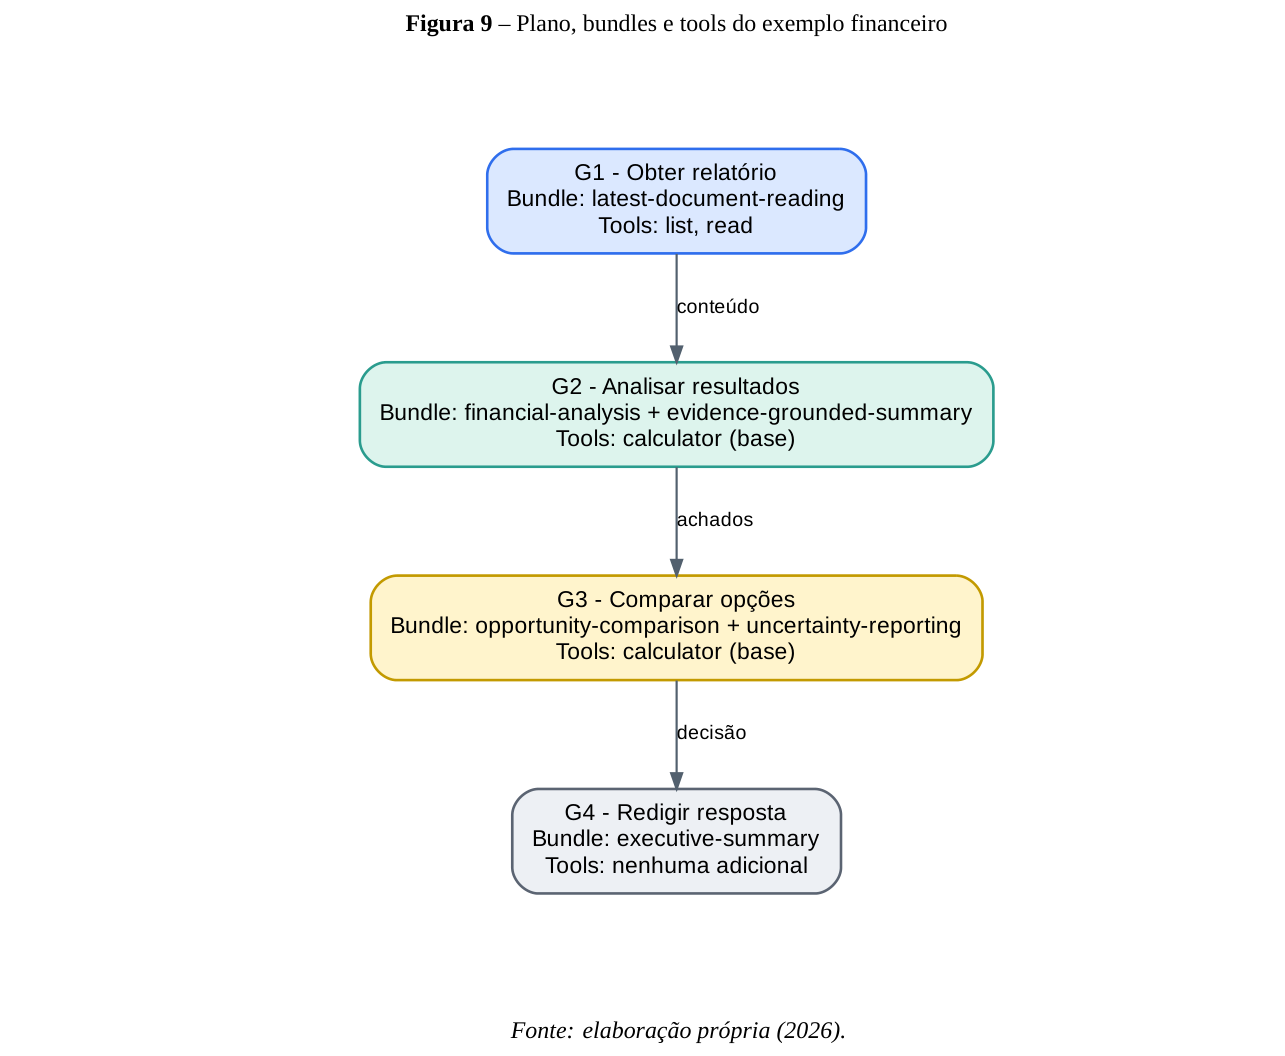
\includegraphics[width=0.97\linewidth]{figures/visual_14_p23.png}
\end{figure}

No primeiro objetivo,\texttt{ latest-document-reading} acrescenta\texttt{ list} e\texttt{ read}. O executor pode listar arquivos, ler cabeçalhos e confirmar o documento sem transformar cada chamada em um nó. No segundo objetivo, duas skills orientam a mesma análise: uma fornece o método financeiro; outra exige que os achados permaneçam ligados às evidências.\texttt{ calculator} está disponível por ser base, mas seu uso não é obrigatório. O terceiro objetivo usa duas skills cognitivas para gerar e comparar alternativas sob incerteza. O quarto organiza a comunicação e produz o conteúdo final. Depois de G4, o compositor apenas empacota o resultado de G4; não executa nova síntese.


\subsection*{7.2 Bundle vazio com tool base}

Pedido:


\textit{Leia o valor bruto da fixture}\texttt{ invoice-028}\textit{ e calcule 17,5\% desse valor.}


% Source PDF page 24

Considere Tbase = \{\texttt{read\_fixture},\texttt{ calculator}\}. O plano pode conter um único objetivo: “produzir o valor derivado correto”. O seletor pode retornar B(g) = ∅, porque ler um identificador conhecido e executar uma operação aritmética não exige um procedimento especializado. O menu permanece capaz de acessar um valor externo e calcular o resultado. Esse exemplo demonstra duas propriedades: skills não são pedágios obrigatórios para qualquer ação, e um caso de validação pode tornar a tool causalmente necessária ao esconder o valor da fixture do prompt. Um cálculo cujo operando já aparece no pedido ilustra apenas disponibilidade, não necessidade empírica de Tbase.


\subsection*{7.3 A mesma tool sob skills diferentes}

\begin{figure}[H]
\centering
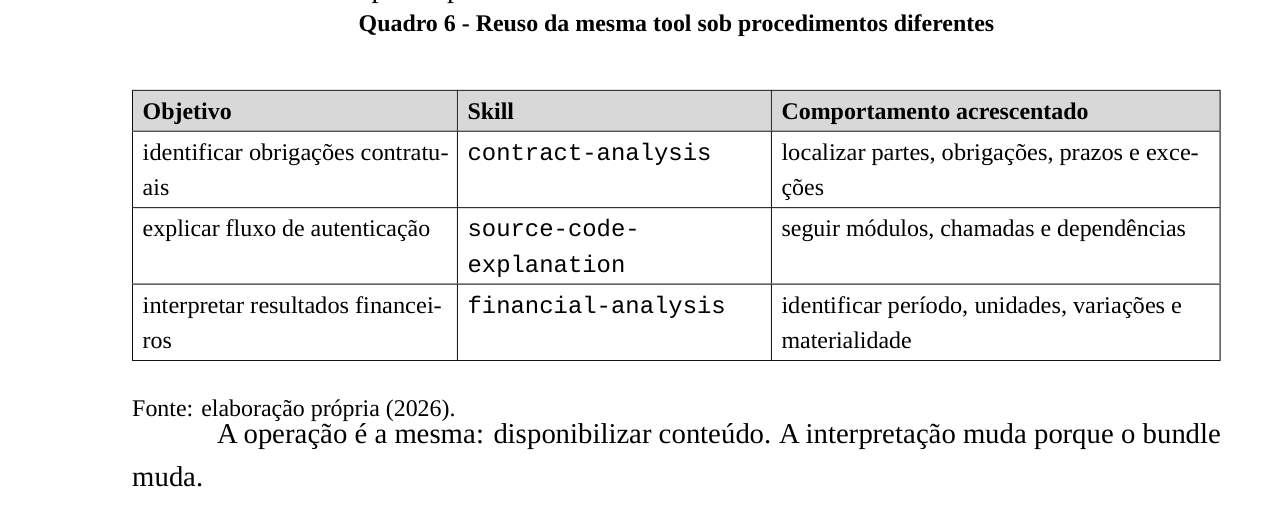
\includegraphics[width=0.97\linewidth]{figures/visual_15_p24.png}
\end{figure}

\subsection*{7.4 Uma skill, várias tools e várias chamadas}

Pedido:


\textit{Encontre o relatório do segundo trimestre e leia as seções de receita e caixa.}


Um único objetivo pode executar a trajetória:


\begin{Verbatim}[breaklines=true,breakanywhere=true,fontsize=\small]
list candidatos
-> read cabeçalho do arquivo A
-> read cabeçalho do arquivo B
-> selecionar o arquivo B
-> read seção de receita
-> read seção de caixa
-> concluir com uma referência ao conteúdo
\end{Verbatim}

O número de chamadas não determina o número de objetivos. O resultado intermediário relevante é “o conteúdo correto está disponível”.


% Source PDF page 25

\subsection*{7.5 Produção e persistência de um artefato}

Pedido:


\textit{Escreva um README de instalação e salve em README.md.}


O plano pode separar:


\noindent 1. produzir o conteúdo do README; 2. persistir o conteúdo em\texttt{ README.md}.\par

A separação não ocorre porque existe a tool\texttt{ write}. Ela ocorre porque há dois resultados observáveis: conteúdo pronto e arquivo persistido. O primeiro objetivo pode usar\texttt{ technical-} \texttt{document-writing} sem tools. O segundo pode usar\texttt{ file-writing}, que declara\texttt{ write}. Se o usuário pedisse apenas “escreva um README”, o segundo objetivo não existiria; a resposta seria entregue no chat.


\section*{8 DECISÕES DE REDUÇÃO E NÃO OBJETIVOS}

\begin{figure}[H]
\centering
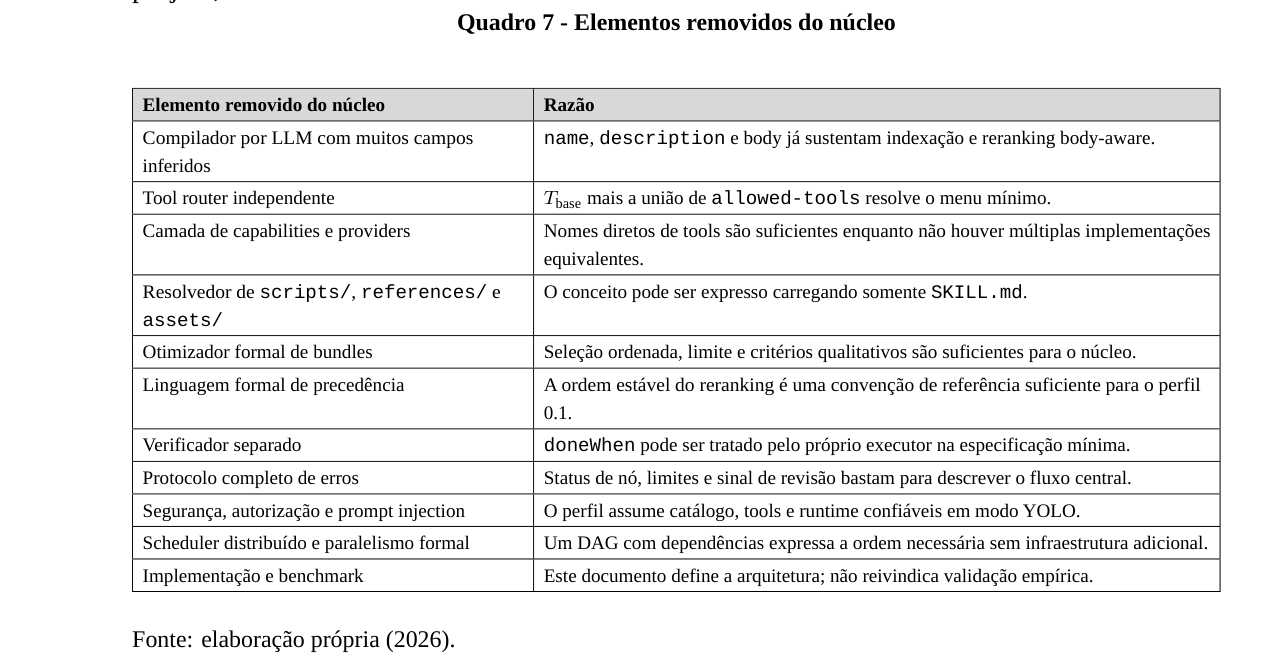
\includegraphics[width=0.97\linewidth]{figures/visual_16_p25.png}
\end{figure}

% Source PDF page 26

\begin{figure}[H]
\centering
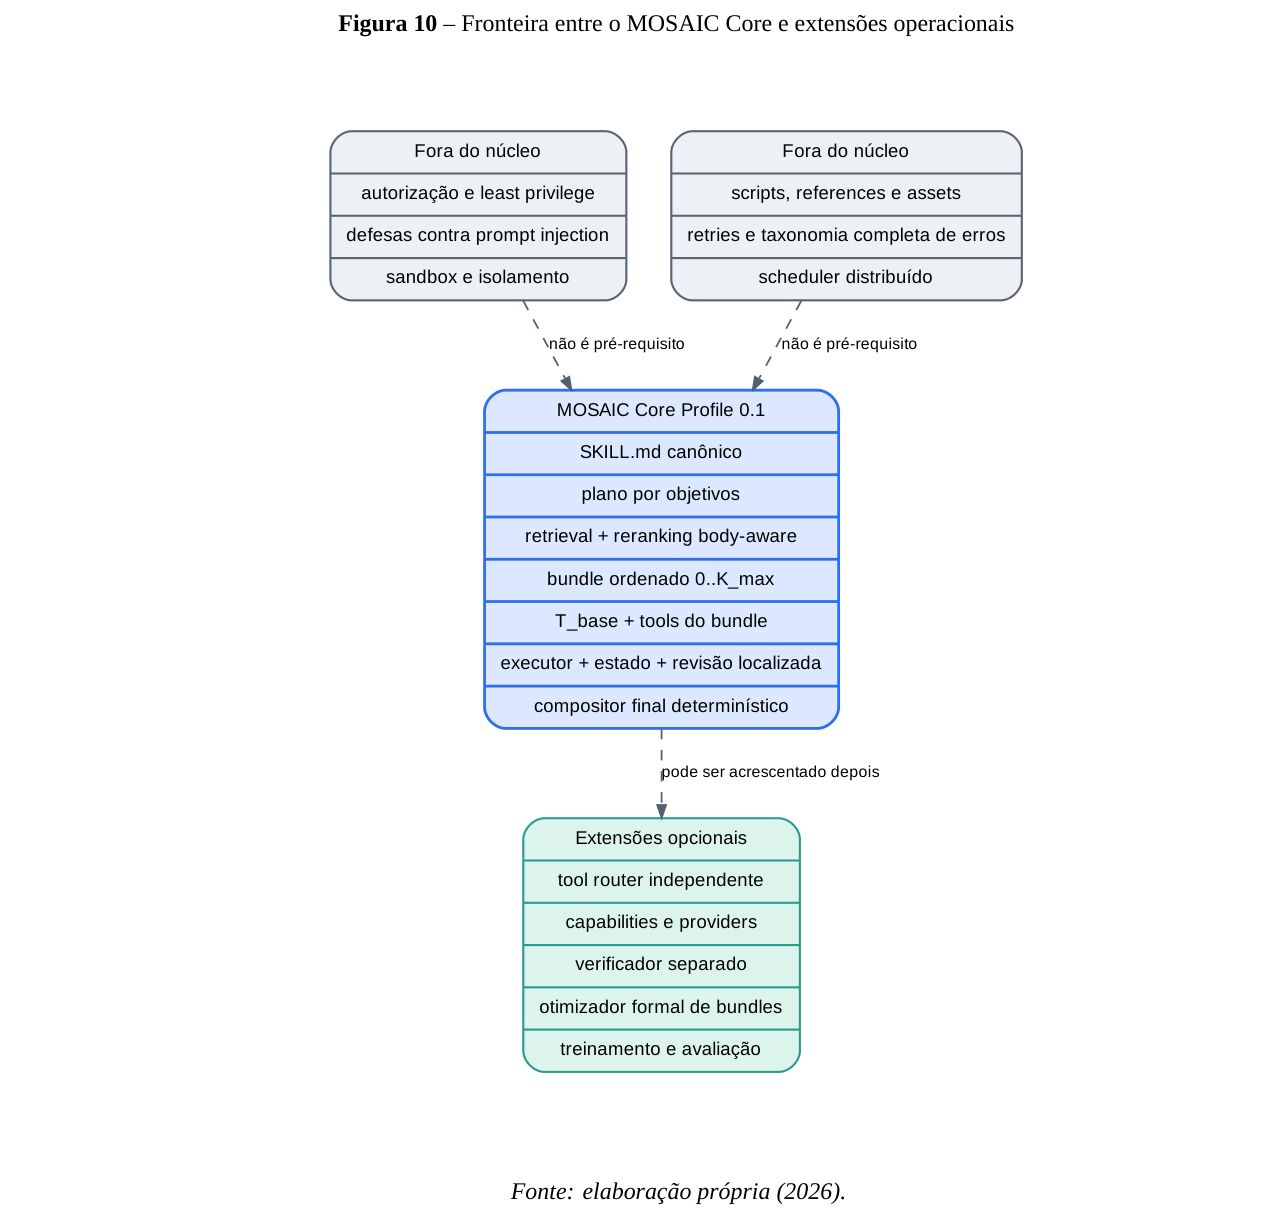
\includegraphics[width=0.97\linewidth]{figures/visual_17_p26.png}
\end{figure}

A fronteira da Figura 10 não impede extensões. Ela estabelece uma ordem: primeiro, tornar a composição conceitualmente clara e implementável; depois, acrescentar mecanismos que casos reais justifiquem. Uma implementação endurecida pode envolver o MOSAIC Core com política, sandbox, filtragem de tools e observabilidade sem alterar a relação fundamental entre objetivo, bundle, menu e executor.


% Source PDF page 27

\section*{9 DISCUSSÃO E LIMITAÇÕES}

\subsection*{9.1 Ausência de validação empírica}

O artigo apresenta uma especificação técnica. Não demonstra que bundles superam top-1, que o feedback do catálogo melhora planos ou que a fórmula de tools produz maior sucesso. Essas são hipóteses decorrentes do desenho e exigem implementação e avaliação separadas. As formulações do texto devem ser lidas como propriedades da arquitetura, não como resultados experimentais.


\subsection*{9.2 Dependência do modelo}

Planner, reranker, seletor e executor dependem da capacidade do modelo de seguir instruções e distinguir comportamentos próximos. Um modelo fraco pode produzir objetivos inadequados, incluir skills redundantes ou ignorar partes do bundle. O MOSAIC organiza o problema, mas não elimina a dependência da competência do modelo.


\subsection*{9.3 Qualidade e tamanho dos bodies}

Retrieval e execução dependem da qualidade do\texttt{ SKILL.md}. Um body vago produz sinal vago. Como o núcleo carrega bodies completos, skills excessivamente longas aumentam custo e podem diluir atenção. A resposta mínima é disciplinar a autoria e manter Kmax pequeno. Compressão automática e carregamento seletivo são extensões, não componentes centrais.


\subsection*{9.4 Conflitos e ordem}

O seletor evita conflitos de forma qualitativa e preserva a ordem do reranking, com desempate determinístico. Isso torna a implementação comparável, mas não garante que a ordem seja ótima quando instruções possuem tensão implícita. Uma linguagem formal de precedência pode ser necessária em catálogos maiores, porém pertence a um perfil posterior se evidência empírica justificar o custo.


\subsection*{9.5 Menu simples de tools}

Tbase pode expor tools que o objetivo não usa. No perfil YOLO máximo, todas as tools ficam visíveis. Essa escolha prioriza simplicidade conceitual e resolve o caso de bundle vazio com tool. Filtragem por estado, custo, causalidade ou risco pertence a arquiteturas de menu mais sofisticadas.


% Source PDF page 28

\subsection*{9.6 Subconjunto de Agent Skills}

O perfil não executa scripts nem carrega referências e assets. Skills que dependem desses recursos não são integralmente executáveis pelo núcleo. Essa restrição é explícita e evita que o artigo prometa uma camada de resolução que não participa da ideia central.


\subsection*{9.7 Revisão localizada}

O sinal de revisão pressupõe que o executor reconheça quando uma observação altera o plano, e que o planner preserve resultados concluídos. A máquina de estados e os contratos tornam o comportamento verificável, mas não garantem que o modelo identifique corretamente todos os triggers.


\subsection*{9.8 Contratos mínimos não substituem operação de produção}

Os contratos do perfil resolvem ambiguidade entre implementações, mas não especificam persistência distribuída, consistência transacional, retries, idempotência, observabilidade com- pleta ou recuperação de infraestrutura. Eles definem o que deve ser trocado entre os componentes, não como cada componente deve ser operacionalizado.


\section*{10 CONSIDERAÇÕES FINAIS}

O MOSAIC Core parte de uma distinção simples: objetivos descrevem resultados, skills ensinam comportamentos, tools executam operações e o modelo interpreta, decide e transforma informações. A partir dela, a arquitetura substitui a associação um-para-um por relações many- to-many. Para cada objetivo, o runtime recupera skills usando o body completo, seleciona um bundle ordenado de zero a várias instruções e monta um menu composto por Tbase e pelas tools declaradas no bundle. O planner recebe uma única passagem de feedback do catálogo antes da execução, e o estado pode provocar revisões localizadas quando novas observações mudam a tarefa.


A revisão 0.1 torna explícitos os contratos de catálogo, plano, estado, bundle, contexto e resultado de nó; define uma máquina de estados mínima; separa Kretrieve, Khint e Kmax; normaliza \texttt{allowed-tools}; projeta o estado por dependência causal; e elimina a duplicidade entre um objetivo de redação e uma segunda síntese final. Essas decisões aumentam a implementabilidade sem acrescentar novos subsistemas à tese. A principal decisão permanece negativa: não acrescentar componentes que não sejam necessários para expressar o fluxo. Não há compilador semântico obrigatório, tool router inde- pendente, camada de providers, resolvedor de recursos, solver de bundles, verificador separado ou protocolo operacional completo. O perfil assume execução YOLO e explicita seus limites. Com essa redução, a tese arquitetural pode ser enunciada de forma direta:


% Source PDF page 29

\textit{A granularidade do plano deve seguir resultados intermediários; a granularidade das} \textit{instruções e das operações deve permanecer composicional dentro de cada objetivo.}


\section*{REFERÊNCIAS}

AGENT SKILLS.\textbf{ Specification}. [S. l.], 2026. Disponível em: https://agentskills.io/specification. Acesso em: 29 jul. 2026. BABU, Rahul Suresh; IYER, Laxmipriya Ganesh. ToolMenuBench: benchmarking tool-menu filtering strategies for reliable and efficient LLM agents.\textbf{ arXiv}, 2026. DOI: 10.48550/ar- Xiv.2606.15508. CHO, Hongcheol; KANG, Ryangkyung; KIM, Youngeun. SkillRet: a large-scale benchmark for skill retrieval in LLM agents.\textbf{ arXiv}, 2026. DOI: 10.48550/arXiv.2605.05726. GAO, Xueping. Compositional skill routing for LLM agents: decompose, retrieve, and compose. \textbf{arXiv}, 2026. DOI: 10.48550/arXiv.2606.18051. GONG, Jingzhi et al. SkillMOO: multi-objective optimization of agent skills for software engineering.\textbf{ arXiv}, 2026. DOI: 10.48550/arXiv.2604.09297. LI, Xiangyi et al. SkillsBench: benchmarking how well agent skills work across diverse tasks. \textbf{arXiv}, 2026. DOI: 10.48550/arXiv.2602.12670. SCHICK, Timo et al. Toolformer: language models can teach themselves to use tools. In: ADVANCES IN NEURAL INFORMATION PROCESSING SYSTEMS, 36., 2023. \textbf{Proceedings [...]} [S. l.]: Curran Associates, 2023. Disponível em: https://arxiv.org/abs/ 2302.04761. Acesso em: 29 jul. 2026. YAO, Shunyu et al. ReAct: synergizing reasoning and acting in language models. In: INTERNA- TIONAL CONFERENCE ON LEARNING REPRESENTATIONS, 2023.\textbf{ Proceedings} \textbf{[...]} [S. l.]: ICLR, 2023. DOI: 10.48550/arXiv.2210.03629. ZHENG, YanZhao et al. SkillRouter: retrieve-and-rerank skill selection for LLM agents at scale. \textbf{arXiv}, 2026. DOI: 10.48550/arXiv.2603.22455.


% Source PDF page 30

\section*{APÊNDICE A - CONTRATOS NORMATIVOS DO RUNTIME}

Este apêndice define a informação mínima que deve atravessar as fronteiras do runtime. Os


\begin{figure}[H]
\centering
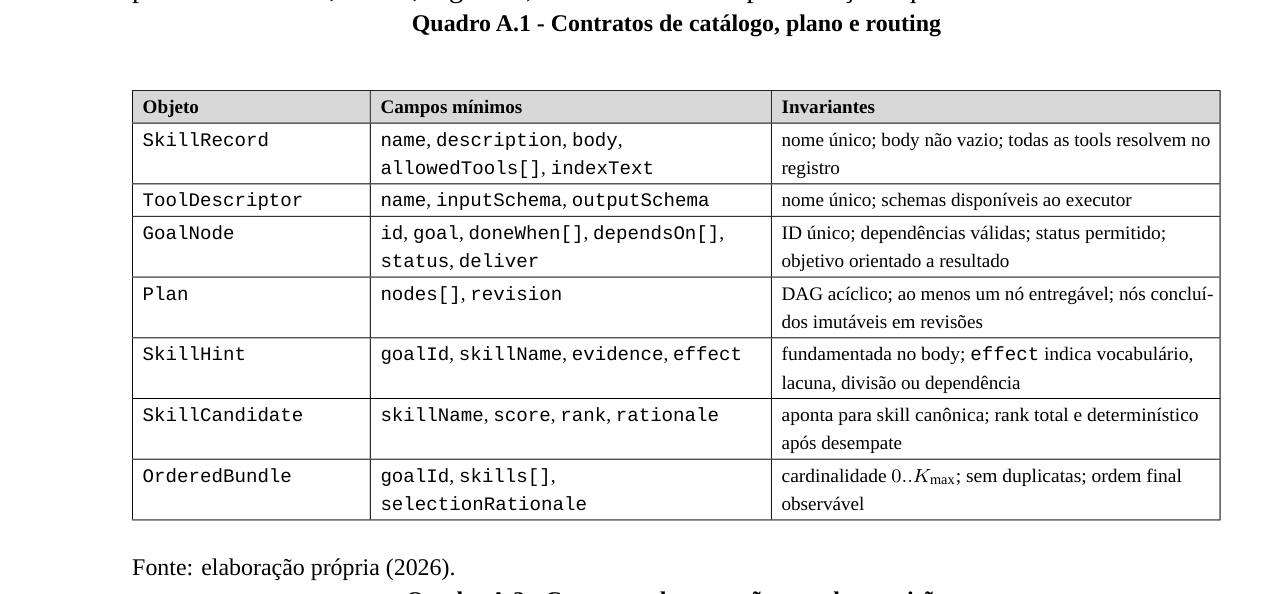
\includegraphics[width=0.97\linewidth]{figures/visual_18_p30.png}
\end{figure}

\begin{figure}[H]
\centering
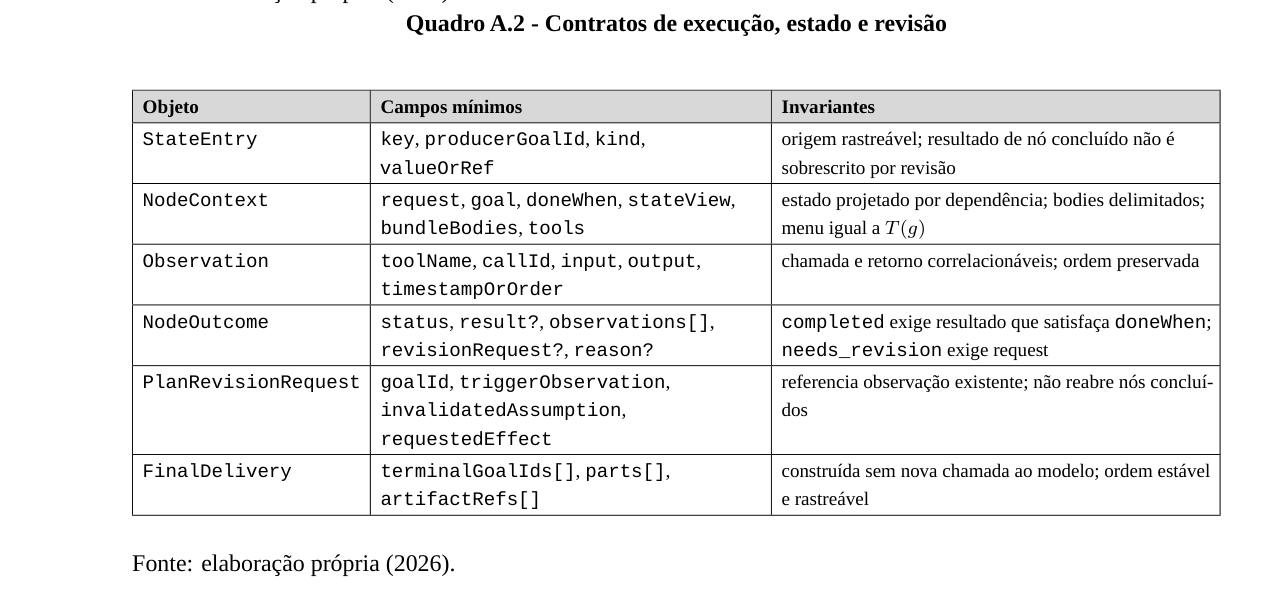
\includegraphics[width=0.97\linewidth]{figures/visual_19_p30.png}
\end{figure}

\textbf{A.1 Validações normativas}


Antes da execução, o runtime deve verificar:


\noindent 1. unicidade de nomes de skills e tools; 2. resolução de cada item de\texttt{ allowed-tools}; 3. unicidade de IDs de objetivos; 4. existência de todas as dependências;\par

% Source PDF page 31

\noindent 5. aciclicidade do plano; 6. Tbase ⊆Tregistry; 7. 0 ≤|B(g)| ≤Kmax; 8. existência de pelo menos um resultado terminal entregável.\par

\textbf{A.2 Semântica de revisão do nó atual}


Quando um nó\texttt{ running} produz\texttt{ needs\_revision}, o planner pode mantê-lo, substituí-lo ou inserir predecessores. Se o nó for mantido, seu ID permanece e seu status retorna a\texttt{ pending}. Se for substituído, o ID antigo não pode ser reutilizado para outro significado. Nenhum resultado parcial é promovido a resultado concluído, embora observações possam permanecer no estado para orientar a revisão.


% Source PDF page 32

\section*{APÊNDICE B - CHECKLIST DE CONFORMIDADE MOSAIC CORE 0.1}

\begin{figure}[H]
\centering
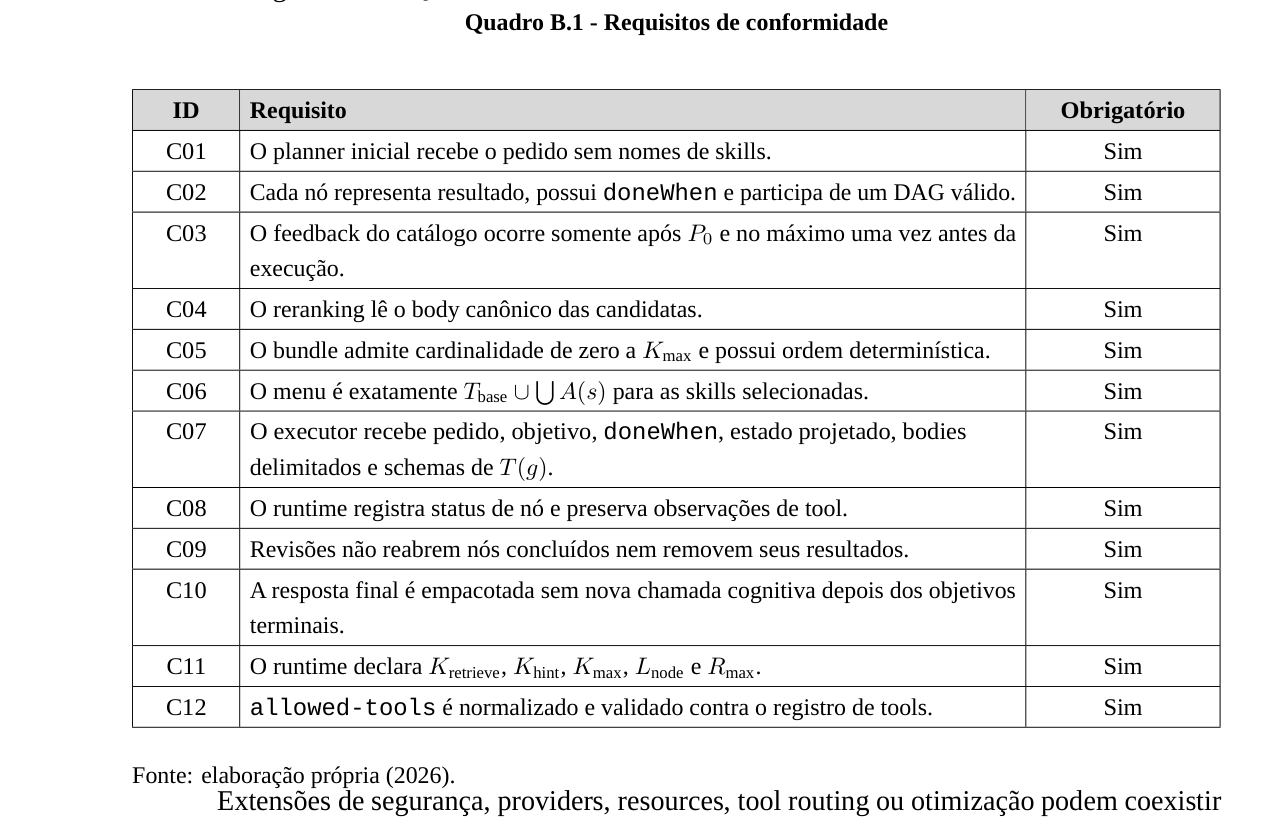
\includegraphics[width=0.97\linewidth]{figures/visual_20_p32.png}
\end{figure}

com o perfil, desde que não alterem silenciosamente esses contratos. Quando alterarem, a imple- mentação deve declarar um perfil derivado em vez de usar o rótulo Core 0.1 sem qualificação.


\end{document}
